\documentclass[../../main.tex]{subfiles}

 \lhead{Implementation: Software}
 
\begin{document}
\lstset{language=Java} 
	\subsection{Software}
	\label{software}
		
		%Overall idea
		As a software patch was already in use with the \ac{VSS}, the idea was to extend this software patch to accommodate the newly proposed functionality. This section will first give a quick overview of the original max patch and then an overview of the newly produced software with a simple explanation of how it works, followed by a more detailed explanation of how the two main parts of the software work.

		The software described was run on a 2012 Mac mini with 16GB of RAM, an IntelCore i7 processor running OSX 10.10.4.

		\subsubsection{Software Overview}

			\paragraph{The Original Patch}
			\label{softwareoverview:original}
				The original max patch was used to convolve a real time audio signal with a set of four \ac{RIR}'s simultaneously, allowing the user to turn their head in the \ac{VAE} through the use of an Oculus Rift as a head tracking device. Four positions within the \ac{VAE} were available. To select one, the user (or an operator) selected an `open' button which prompted a file navigation window. The \ac{RIR} files then had to be found (in the correct order) and opened one at a time, with a new file window opening after each file had been selected. A screen shot of this process is shown in figure~\ref{original}. This was the primary aspect of the original patch that needed extending to make the process automatic.

					%-------------Max UI Flow diagram-------------%
				\begin{figure}[H]
					\centerline{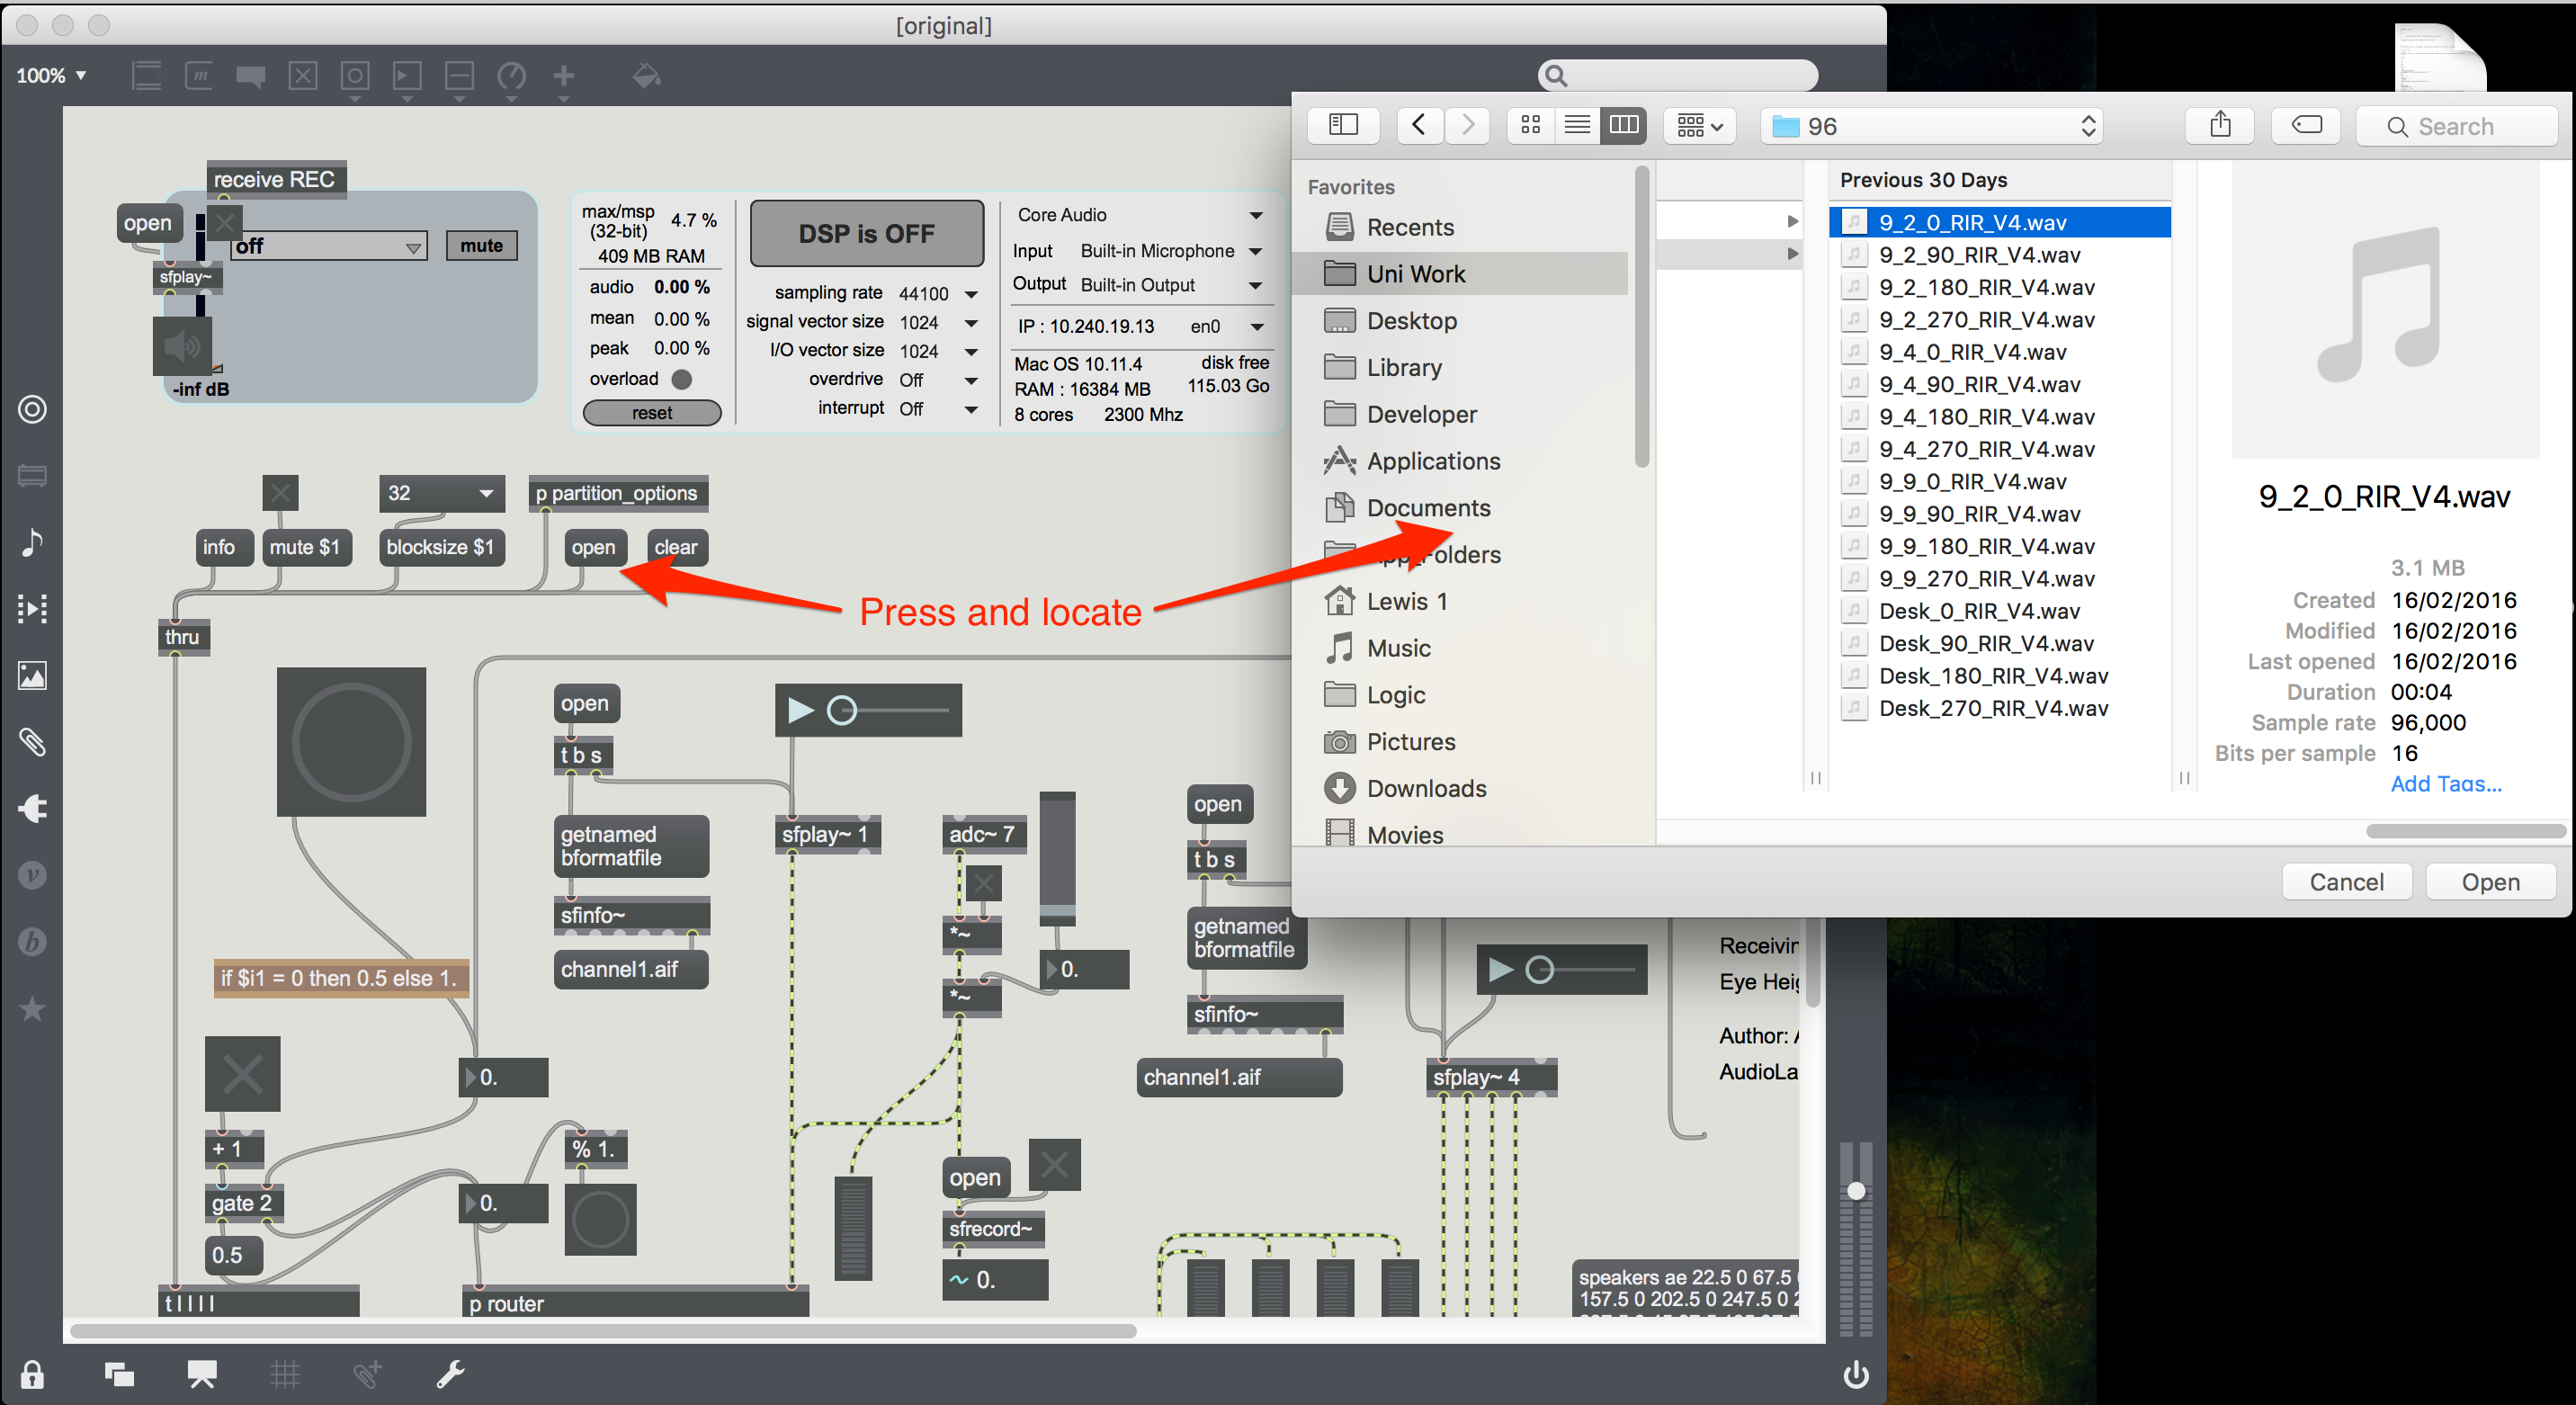
\includegraphics[scale = 0.3]{Sections/Implementation/Max/images/Max/OriginalPatch_Edit.png}}
					\caption{Original Max patch used in the \ac{VSS} showing the file location window that pops up 4 times.}
					\label{original}
				\end{figure}

			\paragraph{Extended Patch Overview}
				Figure~\ref{myPatch} shows an annotated top level view of the Max patch produced to take a user input, load the appropriate \ac{RIR} files and convolve with a real time audio input. The annotated sections can be described as follows:

				\textbf{1:} Two buttons used to reset the system and start the timer used when moving around the space. The settings patch extends to provide a range of options including the density of 

				\textbf{2:} Here, an audio file can be loaded into the system and used instead of a real time audio input. This is used in user test \#3.

				\textbf{3:} A timer system used to synchronise the output of data transfer (from \textbf{4.2} to \textbf{4.3}), panning between convolved audio and the movement of the user interface feedback system (see section~\nameref{locationtracking}).

				\textbf{4.1:} Patches that send a user interface to an iPad which allows a user to select a location within the \ac{VAE}. User interaction is monitored (in the form of screen coordinates) and sent to \textbf{4.2}.

				\textbf{4.2:} Takes the coordinates of the user input and calculates which (if any) \ac{RIR} file should be loaded into the system, in section \textbf{4.3}.

				\textbf{4.3:} Three patches (extended versions of the max explained in section~\nameref{softwareoverview:original}) used to simultaneously convolve an audio signal (real time or audio file) with four directional \ac{RIR} files. While one loads the next necessary \ac{RIR} file the other two are used to simulate the movement of the user by panning the real time audio between the two currently running convolutions. This is how the user is moved along a path, explained in section~\nameref{iteration3}.

				\textbf{5:} An extended version of the real time head-tracking system used in the original patch, used to pan between the four directional \ac{RIR}'s to simulate head movement in the \ac{VAE}.

				%-------------Max UI Flow diagram-------------%
				\begin{figure}[H]
					\centerline{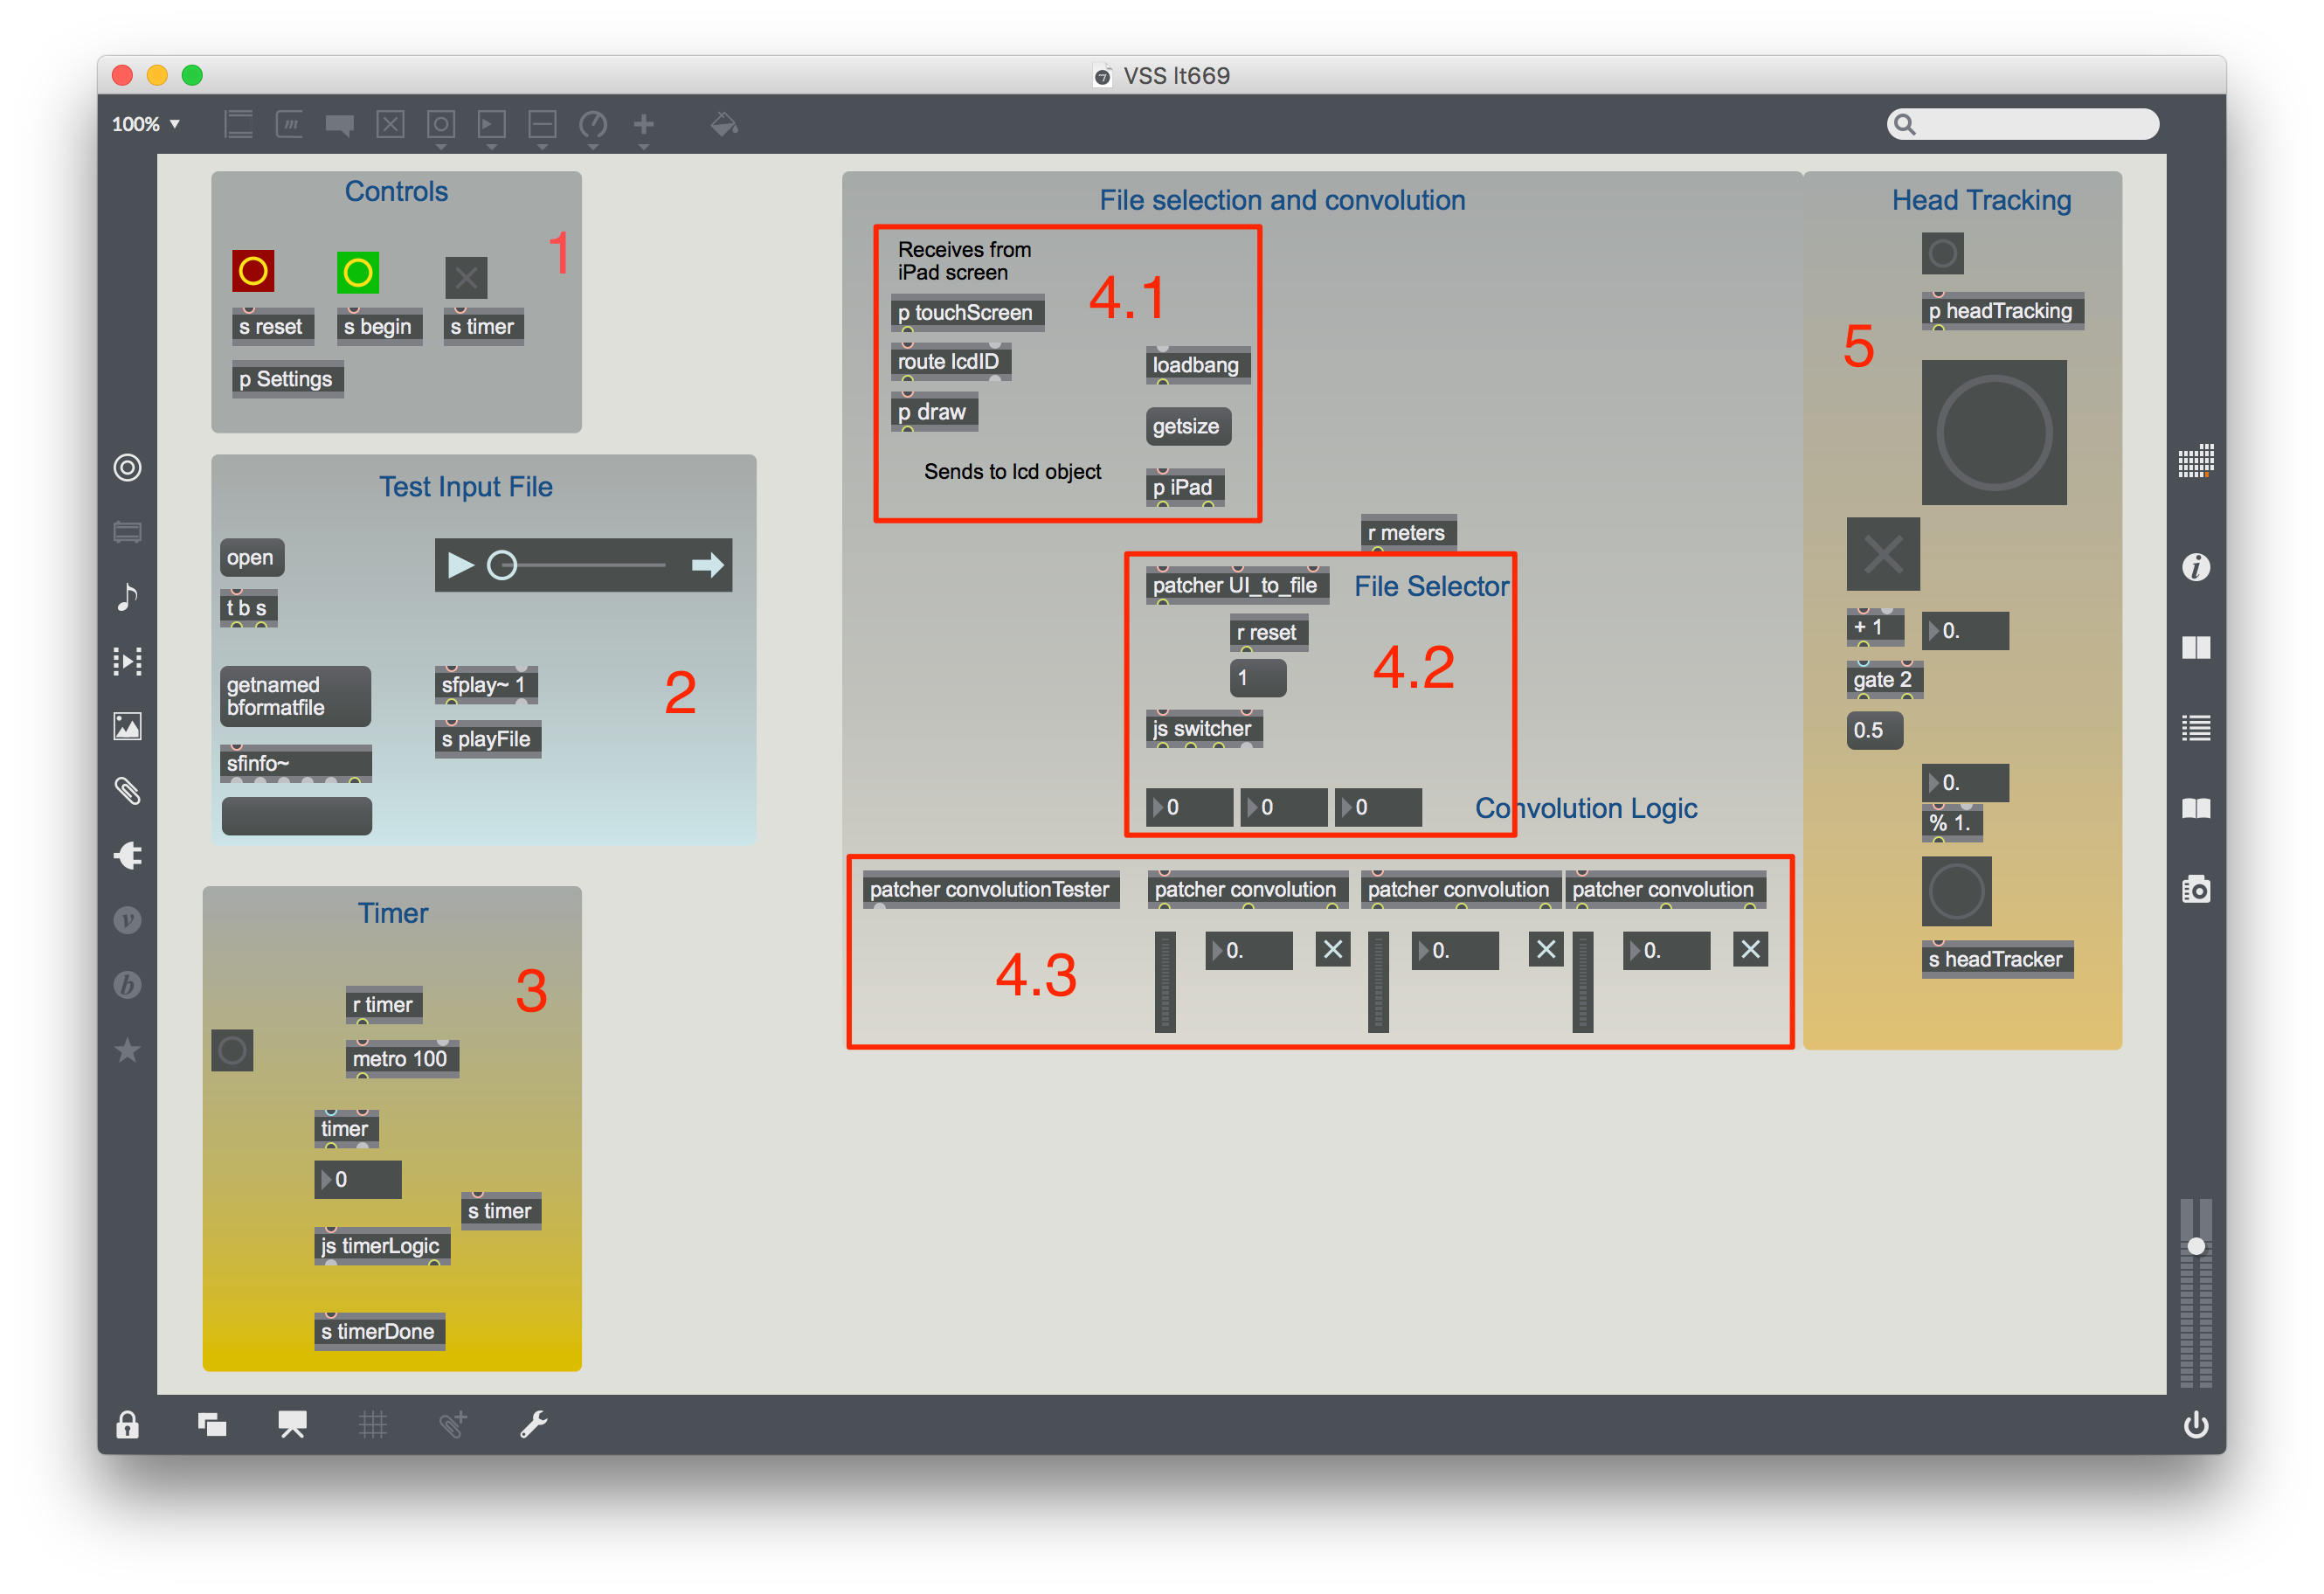
\includegraphics[scale = 0.4]{Sections/Implementation/Max/images/Max/MyPatch_Edit.png}}
					\caption{Top level Max patch}
					\label{myPatch}
				\end{figure}

		

				The software implementation was split into two main sections: \textbf{Location Selection} consisting of section \textbf{4.2} and \textbf{Mobility} mainly consisting of section \textbf{3 and 4.3}.



		\subsubsection{Location Selection}
		\label{locationSelection}
			%User interface section
			%The location selection part of the system was required to present the user with an interface with which they could select a location within the \ac{VAE}. The system would then interpret their input and select the correct \ac{RIR} file(s) to be used in the rest of the system. 

			In order to allow the user to move themselves around the room, they had to be presented with a means of doing so. This involved presenting the user with an interface that resembled the space available to them on which they could select their location. This then had to output the coordinates selected by the user and convert them into a format which can be interpreted as a file name indicating which \ac{RIR} in the available grid to use. This could then be passed to the rest of the system to load the appropriate files. A simple block diagram of the user interface part of the system is shown in figure~\ref{flowDiagram}.


			%-------------Max UI Flow diagram-------------%
			\begin{figure}[H]
				\centerline{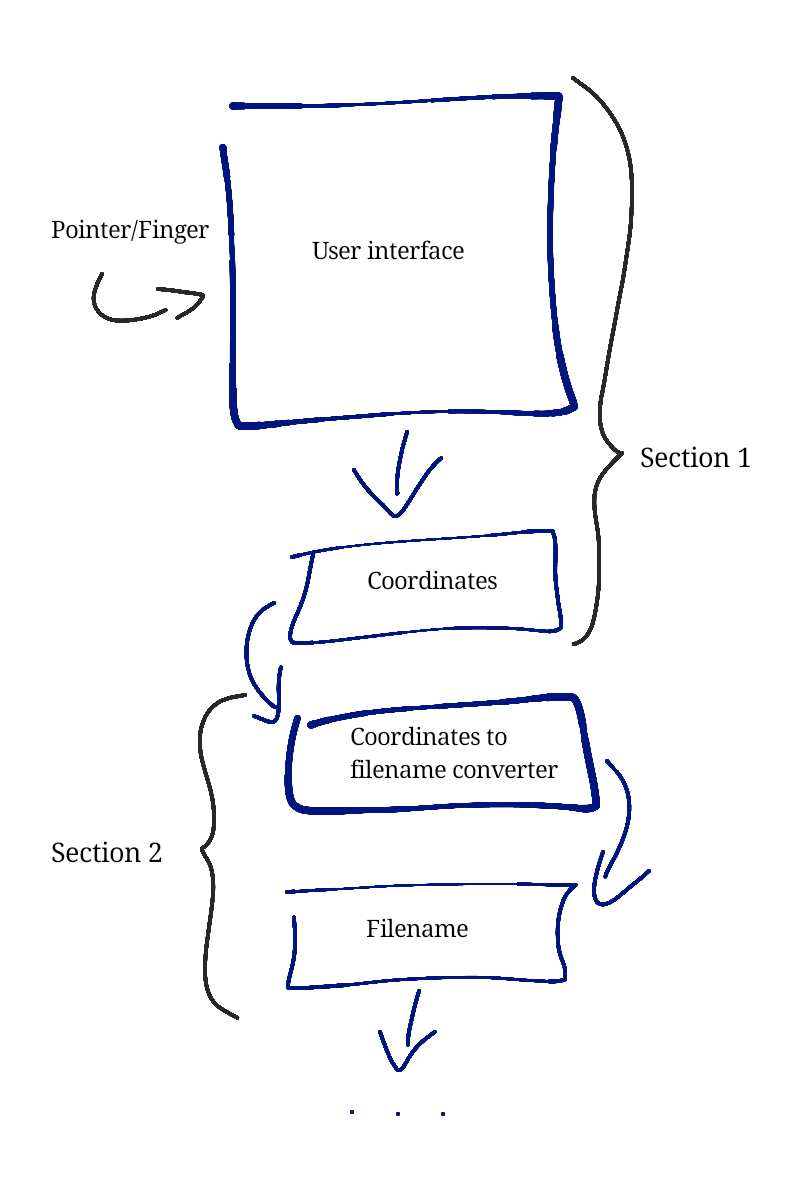
\includegraphics[scale = 0.3]{Sections/Implementation/Max/images/FlowDiagrams/Max1_V2.png}}
				\caption{Flow diagram of the location selection software design. \textbf{Section 1} indicates the user interface section where coordinates are recorded and \textbf{Section 2} takes these coordinates and finds the appropriate \ac{RIR} file.}
				\label{flowDiagram}
			\end{figure}

			In Max, the ‘lcd’ object is used for this function. This object presents a quadrilateral of variable length and height with the ability to output its dimensional information by sending a ‘getSize’ message to its input, as well as output the coordinates of a mouse click/drag. Figure~\ref{lcd} shows the lcd object with its inputs and outputs represented by section 1 in figure~\ref{flowDiagram}.

			%-------------LCD Image-------------%
			\begin{figure}[H]
				\centerline{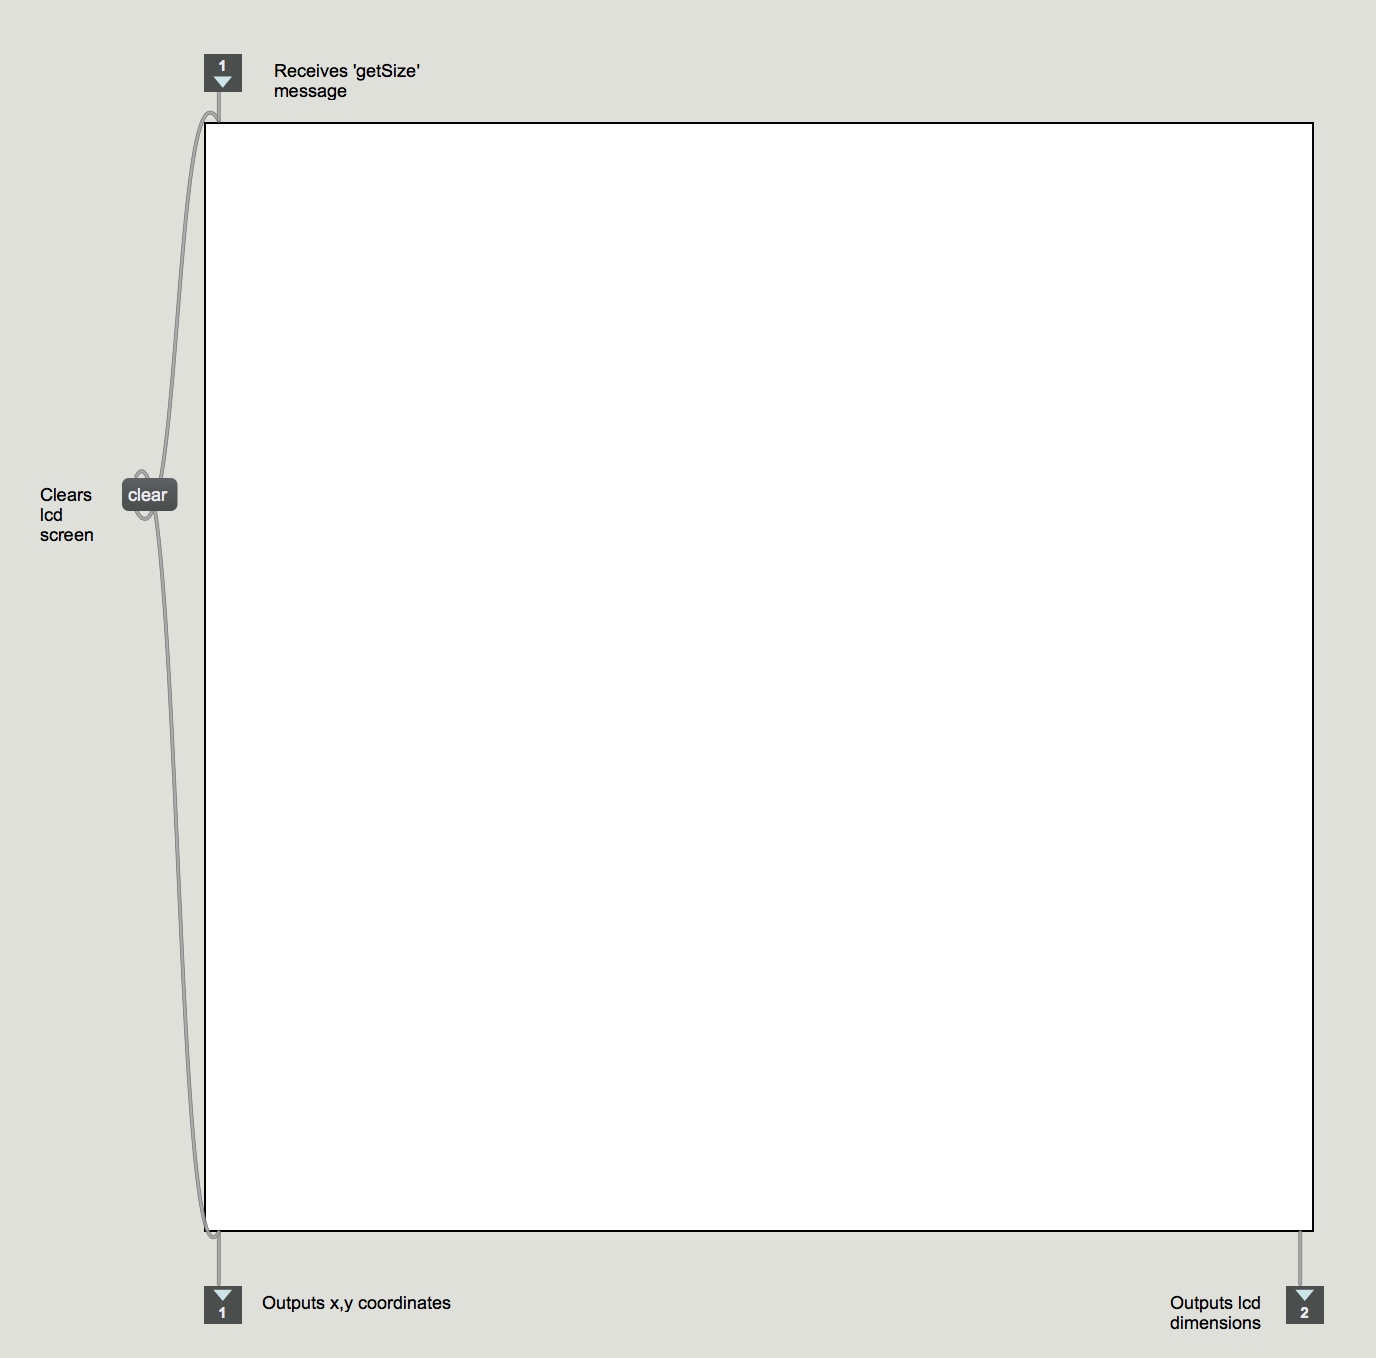
\includegraphics[scale = 0.4]{Sections/Implementation/Max/images/Max/lcd.png}}
				\caption{Flow diagram of the location selection software design}
				\label{lcd}
			\end{figure}

			The outputs from the lcd object are sent to the patch ‘UI\_to\_file’ which contains a JavaScript file called ‘loadFilesLogic’. This JavaScript file converts the (x,y) coordinates into an appropriate file name, by taking into account the size of the lcd screen and how many RIRs there are per meter.

			This lcd screen could also be displayed on an iPad which was used as a remote user interaction. Initially, the more popular and supported application \textbf{Mira} \cite{mira} was going to be used. This allows for the mirroring of a selected portion of a Max patch to be displayed and interacted with on an iPad. However, the lcd object used to track coordinates was not supported by this application and thus did not appear on the iPad. Instead an alternative was found. Cycling74, the same company that produces Max/MSP and Mira also created an app for the iPhone and iPad called c74 \cite{c74} and allows for the creation of an independent interface that can control objects within the max patch. The operation of this section is explained further in section \nameref{locationtracking}

			The javascript takes 5 inputs: UI (x,y) coordinates , (x,y) lcd dimensions and a number representing how many rows and colums of \ac{RIR} locations there should be available. This last value is calculated by sending a number from 1-5 (distance per RIR) to the third inlet of the UI\_to\_file patch (on the far right). As the maximum number of RIRs that will be available per length of the room is 15, 15 is divided by the input and rounded to the nearest integer, giving the number of rows and columns the lcd screen should be split into (the exact number of rows and columns is calculated later in the javascript file). This information can then be used to determine in which \textit{‘section’} (row and column) the user is currently located based on their coordinates, allowing it to load the appropriate RIRs that are available in that section. Figure~\ref{locationsConvert} shows the section of `UI\_to\_file' highlighting each section.

			%-------------UI_to_file Image-------------%
			\begin{figure}[H]
				\centerline{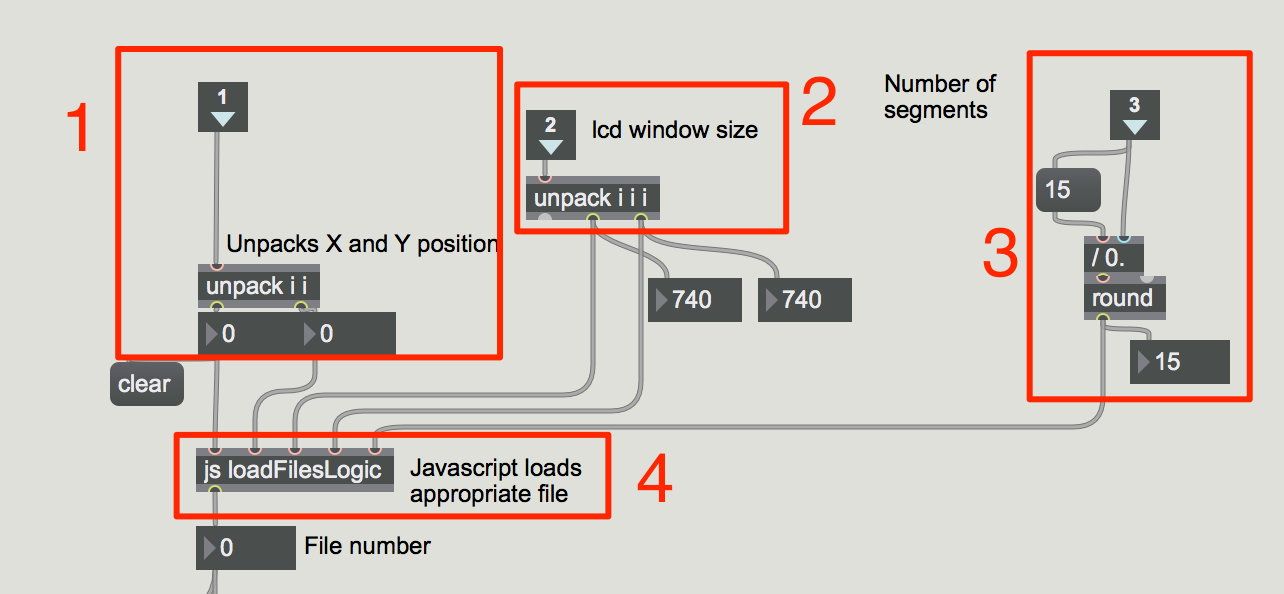
\includegraphics[scale = 0.6]{Sections/Implementation/Max/images/Max/UI_to_file_edit_4.png}}
				\caption{Screen shot from Max showing a section that converts the user interface coordinates into the appropriate file name. 1) Coordinates from lcd object 2) Dimensions of lcd object 3) Number of segments the lcd object should be split into due to the number of \ac{RIR}'s per meter 4) JavaScript file that produces an appropriate file name given the input data.}
				\label{locationsConvert}
			\end{figure}

			\paragraph{File name JavaScript: `loadFilesLogic.js'}

				%-------------Input Code-------------%
				\begin{minipage}{0.6\textwidth}
					\begin{lstlisting}
					function msg_int(input){
						if(inlet == 0){
							xPos = input; 
						} else if (inlet == 1){
							yPos = input;//Add off set to start at (0,1)
						} else if (inlet == 2){
							windowSize [0] = input;
						} else if (inlet == 3){
							windowSize [1] = input;
						} else if(inlet==4){
							numberOfMeters = input;
						}
					\end{lstlisting}
				\end{minipage}
				\begin{minipage}{0.4\textwidth}
					The first section in the JavaScript simply stores the data from different inputs to different variables that are used throughout the rest of the code, where:

					\vspace{5mm}

					\hspace{-10mm}\begin{tabular}{r l}
						xPos & = user x coordinate \\
						yPos & = user y coordinate \\
						windowSize[0] & = lcd length \\
						windowSize[1] & = lcd height \\
						numberOfMeters & = Integer to calculate rows/columns \\
					\end{tabular}
					
				\end{minipage}

				As can be seen in figures~\ref{2m},\ref{3m},\ref{4m} and~\ref{5m} in \nameref{appendixB}, there are not always the same number of rows as there are columns in each of the grids. The if else statements in figure~\ref{jsPosition} calculate the users positions by taking the users x and y coordinates and dividing by the x and y dimensions of the lcd screen, giving a percentage of how far across the room they are. This allows the for lcd screen to be resized allowing it to be used of different sized screens in the future (see section \nameref{furtherwork}). This value is then multiplies by either the number of rows (x axis) or columns (y axis) there are, which is calculated by adding or subtracting 1, or using the value of numberOfRows which is calculated before being input into the js object. The following table indicates how many rows and columns there are given the inputs to the js object:

					\begin{center}
					\begin{tabular}{c c c c c}
						Distance between \ac{RIR}`s (m) & Calculation & numberOfMeters & Rows & Columns\\
						1 & 15/1 & 15 & 15 & 16\\
						2 & 15/2 & 8 & 7 & 8\\
						3 & 15/3 & 5 & 5 & 5\\
						4 & 15/4 & 4 & 3 & 4\\
						5 & 15/5 & 3 & 3 & 3\\
					\end{tabular}
				\end{center}

				Lines 17 and 18, the calculated positions are rounded to the nearest integer in order to determine which \ac{RIR} location the user is closest too. Lines 21 to 26, create an initial offset to prevent the lcd screen from starting at location (0,0), as this is not a physical point in the room itself thus preventing errors from occurring when searching for the appropriate \ac{RIR} file.

				\begin{figure}[H]
				\begin{lstlisting}
					//Split into sections
					if(numberOfMeters == 3 || numberOfMeters == 5){
						//Even grid for 3m and 5m
						xPosition = (xPos/windowSize[0])*(numberOfMeters);
						yPosition = (yPos/windowSize[1])*(numberOfMeters);
					} else if (numberOfMeters == 4 || numberOfMeters == 8){
						//4m separation requires different x,y coordinate scaling
						xPosition = (xPos/windowSize[0])*(numberOfMeters-1);
						yPosition = (yPos/windowSize[1])*(numberOfMeters);
					} else{
						//Extra row for others
						xPosition = (xPos/windowSize[0])*(numberOfMeters); 
						yPosition = (yPos/windowSize[1])*(numberOfMeters+1);
					}	

					//Round to nearest value
					xSection = Math.round(xPosition);
					ySection = Math.round(yPosition); 
					
					//Start the lcd grid sections from column 1 row 1 instead of column 0 row 0
					if(xSection == 0){
						xSection = 1; 
					}
					if(ySection == 0){
						ySection = 1;
					}
					\end{lstlisting}
					\caption{Code used to calculate user location}
					\label{jsPosition}
					\end{figure}

					 The section the user is currently located in is then saved to the first address in a array and can be used to compare against their previous position to check whether a new file needs to be loaded. This is necessary because each time the user touched the user interface, thus changing the x and y coordinates, javascript file is run. However, if there new location is still within the same `section' then a new \ac{RIR} file does not need to be loaded.

					 In figure~\ref{jsFile}, lines 6 to 26 contain one large if statement. This essentially prevents the program from calculating, searching for and trying to load a file if the same one is still in use, thus saving computation time. This is done by comparing the section of the grid the user is currently in with the previous section they were currently in and if it has changed the file name for the new location should be calculated and searched for, otherwise no new file should be calculated.

					 If the location of the user has changed, two more conditions are checked in lines 8 and 14. This ensures that only the section that has changed is updated, ie, if the user has moved to the left, only the X axis section is updated.

					 Finally, the appropriate file name is calculated. Two different algorithms are used depending on which \ac{RIR} grid is being used. Both essentially take the section the user is located on the X axis, and add the number of locations there are due to how many rows down the room they are located.

					 This then outputs a number from 1 to the maximum number of locations in the selected grid.

				
					\begin{figure}[H]
					\begin{lstlisting}
					//Store current location
					xArray[0] = xSection;
					yArray[0] = ySection;

					//If either coordinate is changed search for new files
					if(xArray[0] != xArray[1] || yArray[0] != yArray[1]){
						
						if(xArray[0] != xArray[1]){
							//Store previous value
							xArray[1] = xArray[0];
							X = xArray[0];
						}
						
						if(yArray[0] != yArray[1]){
							yArray[1] = yArray[0];
							Y = yArray[0]
						}
						
						//Output user location within grid
						if(numberOfMeters == 4 || numberOfMeters == 8){
							fileNumber = X + ((numberOfMeters-1)*(Y-1)); //Requires different algorithm for 2m and 4m due to different grid shapes
						} else {
							fileNumber = X + ((numberOfMeters)*(Y-1));
						}	
						outlet(1,fileNumber);
					}
					\end{lstlisting}
					\caption{Code used to search for appropriate file name}
					\label{jsFile}
					\end{figure}
		

		\subsubsection{Mobility Implementation}

		The following sections describe two earlier iterations of the systems that were attempted and the issues faced, eventually leading to the third and final iteration which can been seen as a compromise between system speed and desired functionality. All three iterations are extensions of the original patch used in the \ac{VSS} which use spat to load \ac{RIR} files into the system, and to convolve a real time audio input with them.

		 \paragraph{Iteration 1}
		 \label{iteration1}
		 	%Idea to stay between RIRs in a grid
		 	% Initially, the idea was to pre-load a grid of the closest \ac{RIR} locations that surrounded the user and simultaneously convolve the real-time audio with all of the \ac{RIR} files. This is illustrated on the left in figure~\ref{iteration1Panning} which shows annotated grid positions on the lcd screen labeled 1 - 9. The patch on the right shows the corresponding volume bars used to automatically vary the output level of each of the convolved signals depending on the users position within the defined grid, essentially panning between the grid position, allowing the user to move freely between them.

		 	Initially, the idea was to pre-load a grid of the closest \ac{RIR} locations that surrounded the user and simultaneously convolve the real-time audio with all of the \ac{RIR} files. This is illustrated on the left in figure~\ref{iteration1Panning} which shows annotated grid positions on the lcd screen labeled 1 - 9. The patch on the right shows the corresponding volume bars (also labelled 1 - 9) used to automatically vary the output level of each of the convolved signals. This required a panning algorithm for each of the positions in the defined grid, an overview of which is shown in figure~\ref{iteration1PanningCombined} in \nameref{appendixC}, based on where the user has moved relative to the centre position essentially allowing the user to move freely.

		 	When the user reaches on of the other locations in the grid, that location becomes the centre of a new grid, and the appropriate files are loaded around that centre positions through the use of a javascript file. This requires the system to simultaneously load 4 \ac{RIR} files per location, of which there are 9, meaning 36 files are loaded into the system at once. Due to the time taken to load all of the files, the system ran too slow and could not be used for real time movement.

		 	A video demonstrating the functionality of the proposed system can be found \href{run:./././SupportingFiles/Webpage/pages/video.html}{link} \textbf{HERE} \textbf{LINK!: Writeup/videios/iteration1Panning}.

		 	%-------------Iteration1 Panning Image-------------%
			\begin{figure}[H]
				\centerline{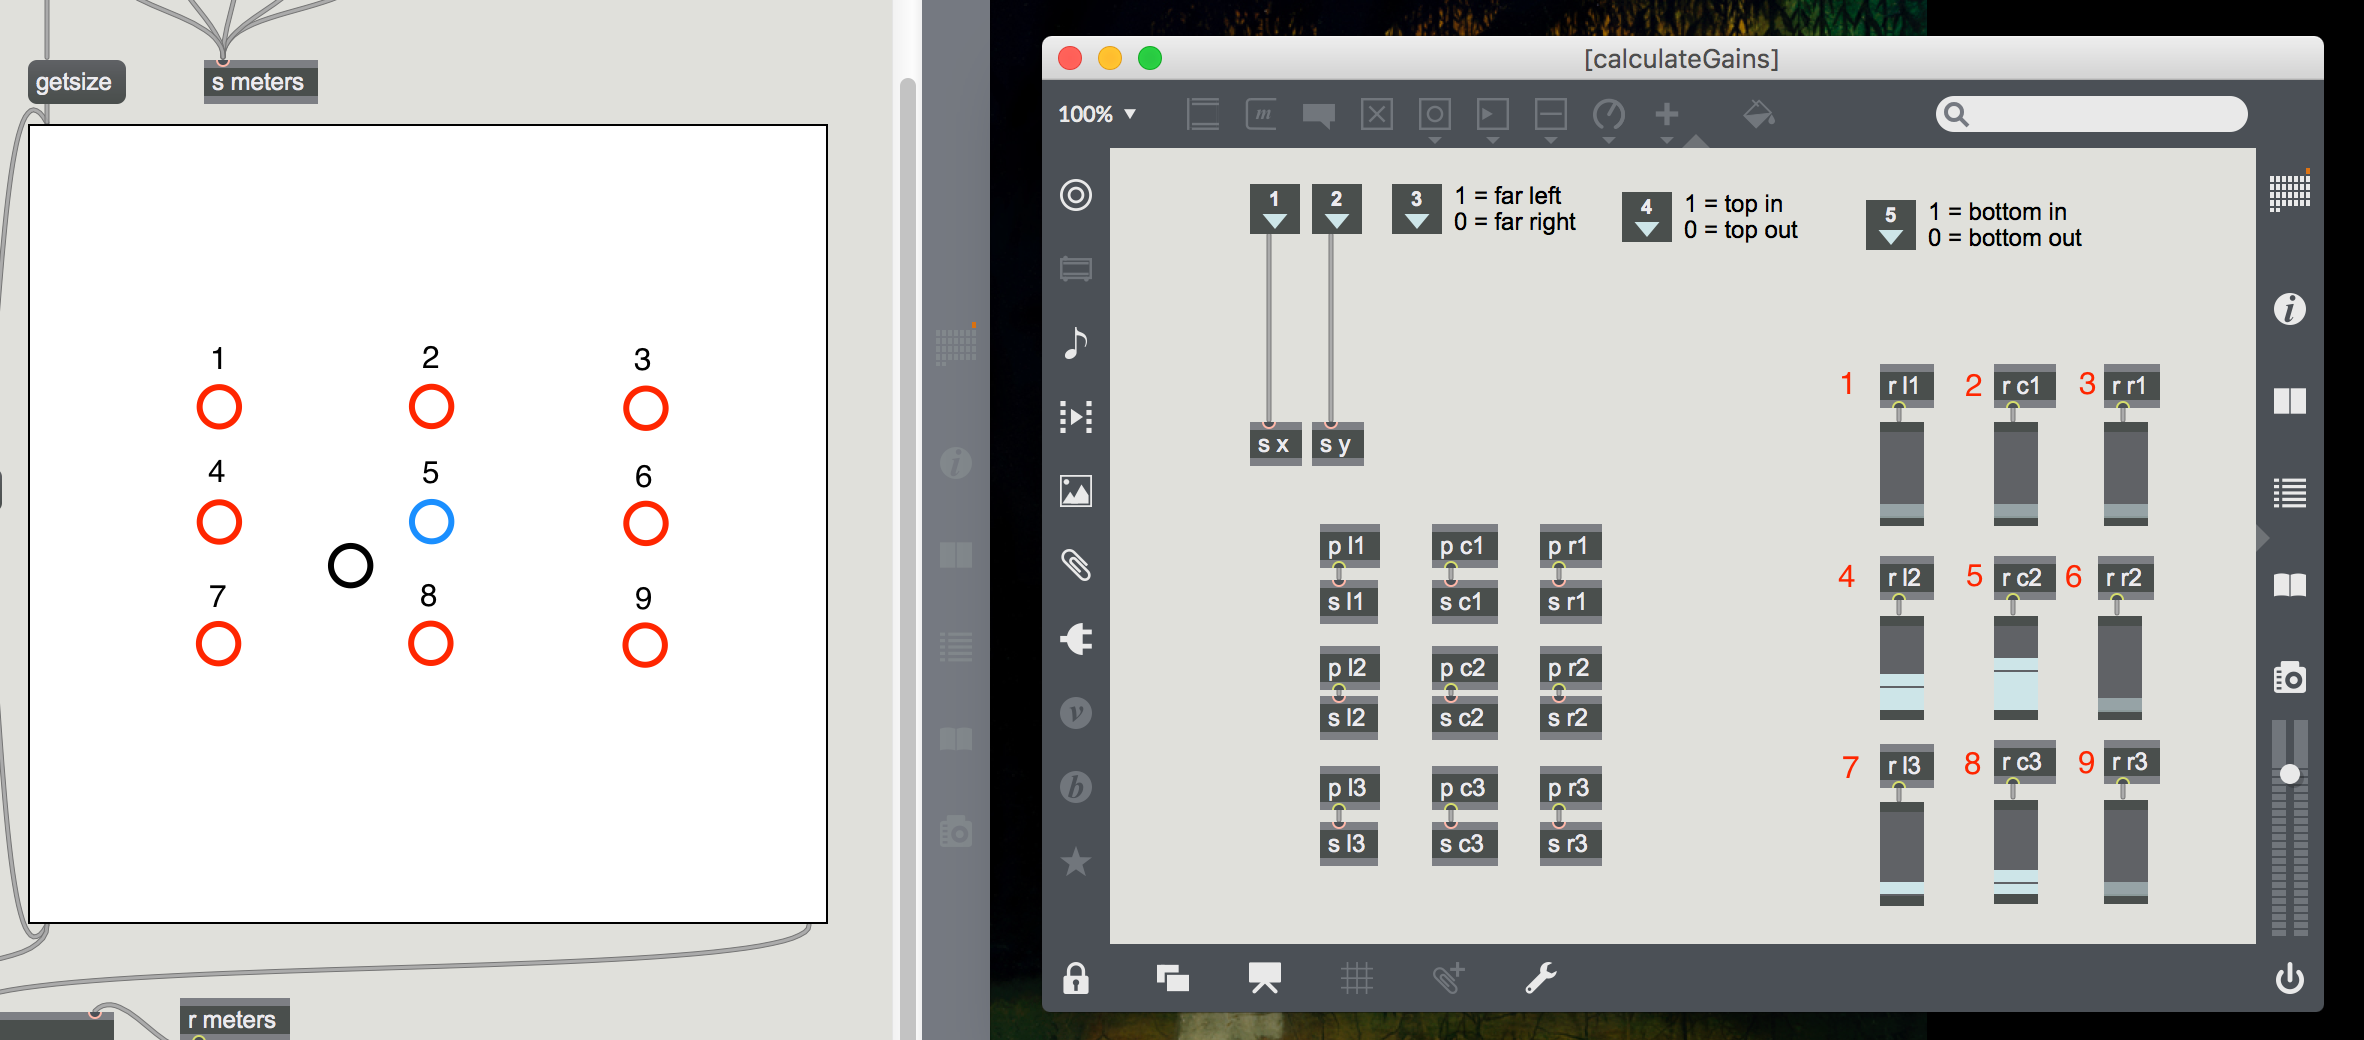
\includegraphics[scale = 0.45]{Sections/Implementation/Max/images/Max/iteration1/panning_edit2.png}}
				\caption{}
				\label{iteration1Panning}
			\end{figure}


		 	%Loading issued

		 \paragraph{Iteration 2}
		 	%Preload RIRs

		 	In an attempt to maintain the current implementation and solve the file loading time issue, a patch was built to pre-load all the \ac{RIR} files, meaning the files only had to be associated with a grid position as opposed to loaded every time a new position was used. This involved running a convolution patch for each file loaded into the system. As the files would no longer need to be loaded into the system, the user interface section described in section~\nameref{locationSelection} is used to decide which of the convolution patched to bypass and mute, and which ones to run. This means that only the grid of \ac{RIR}'s being used would be convolved with the audio signal, saving computational resources. Figure~\ref{preload} shows part of the patch used to pre-load all the \ac{RIR} files.

		 	%-------------Preload Image-------------%
			\begin{figure}[H]
				\centerline{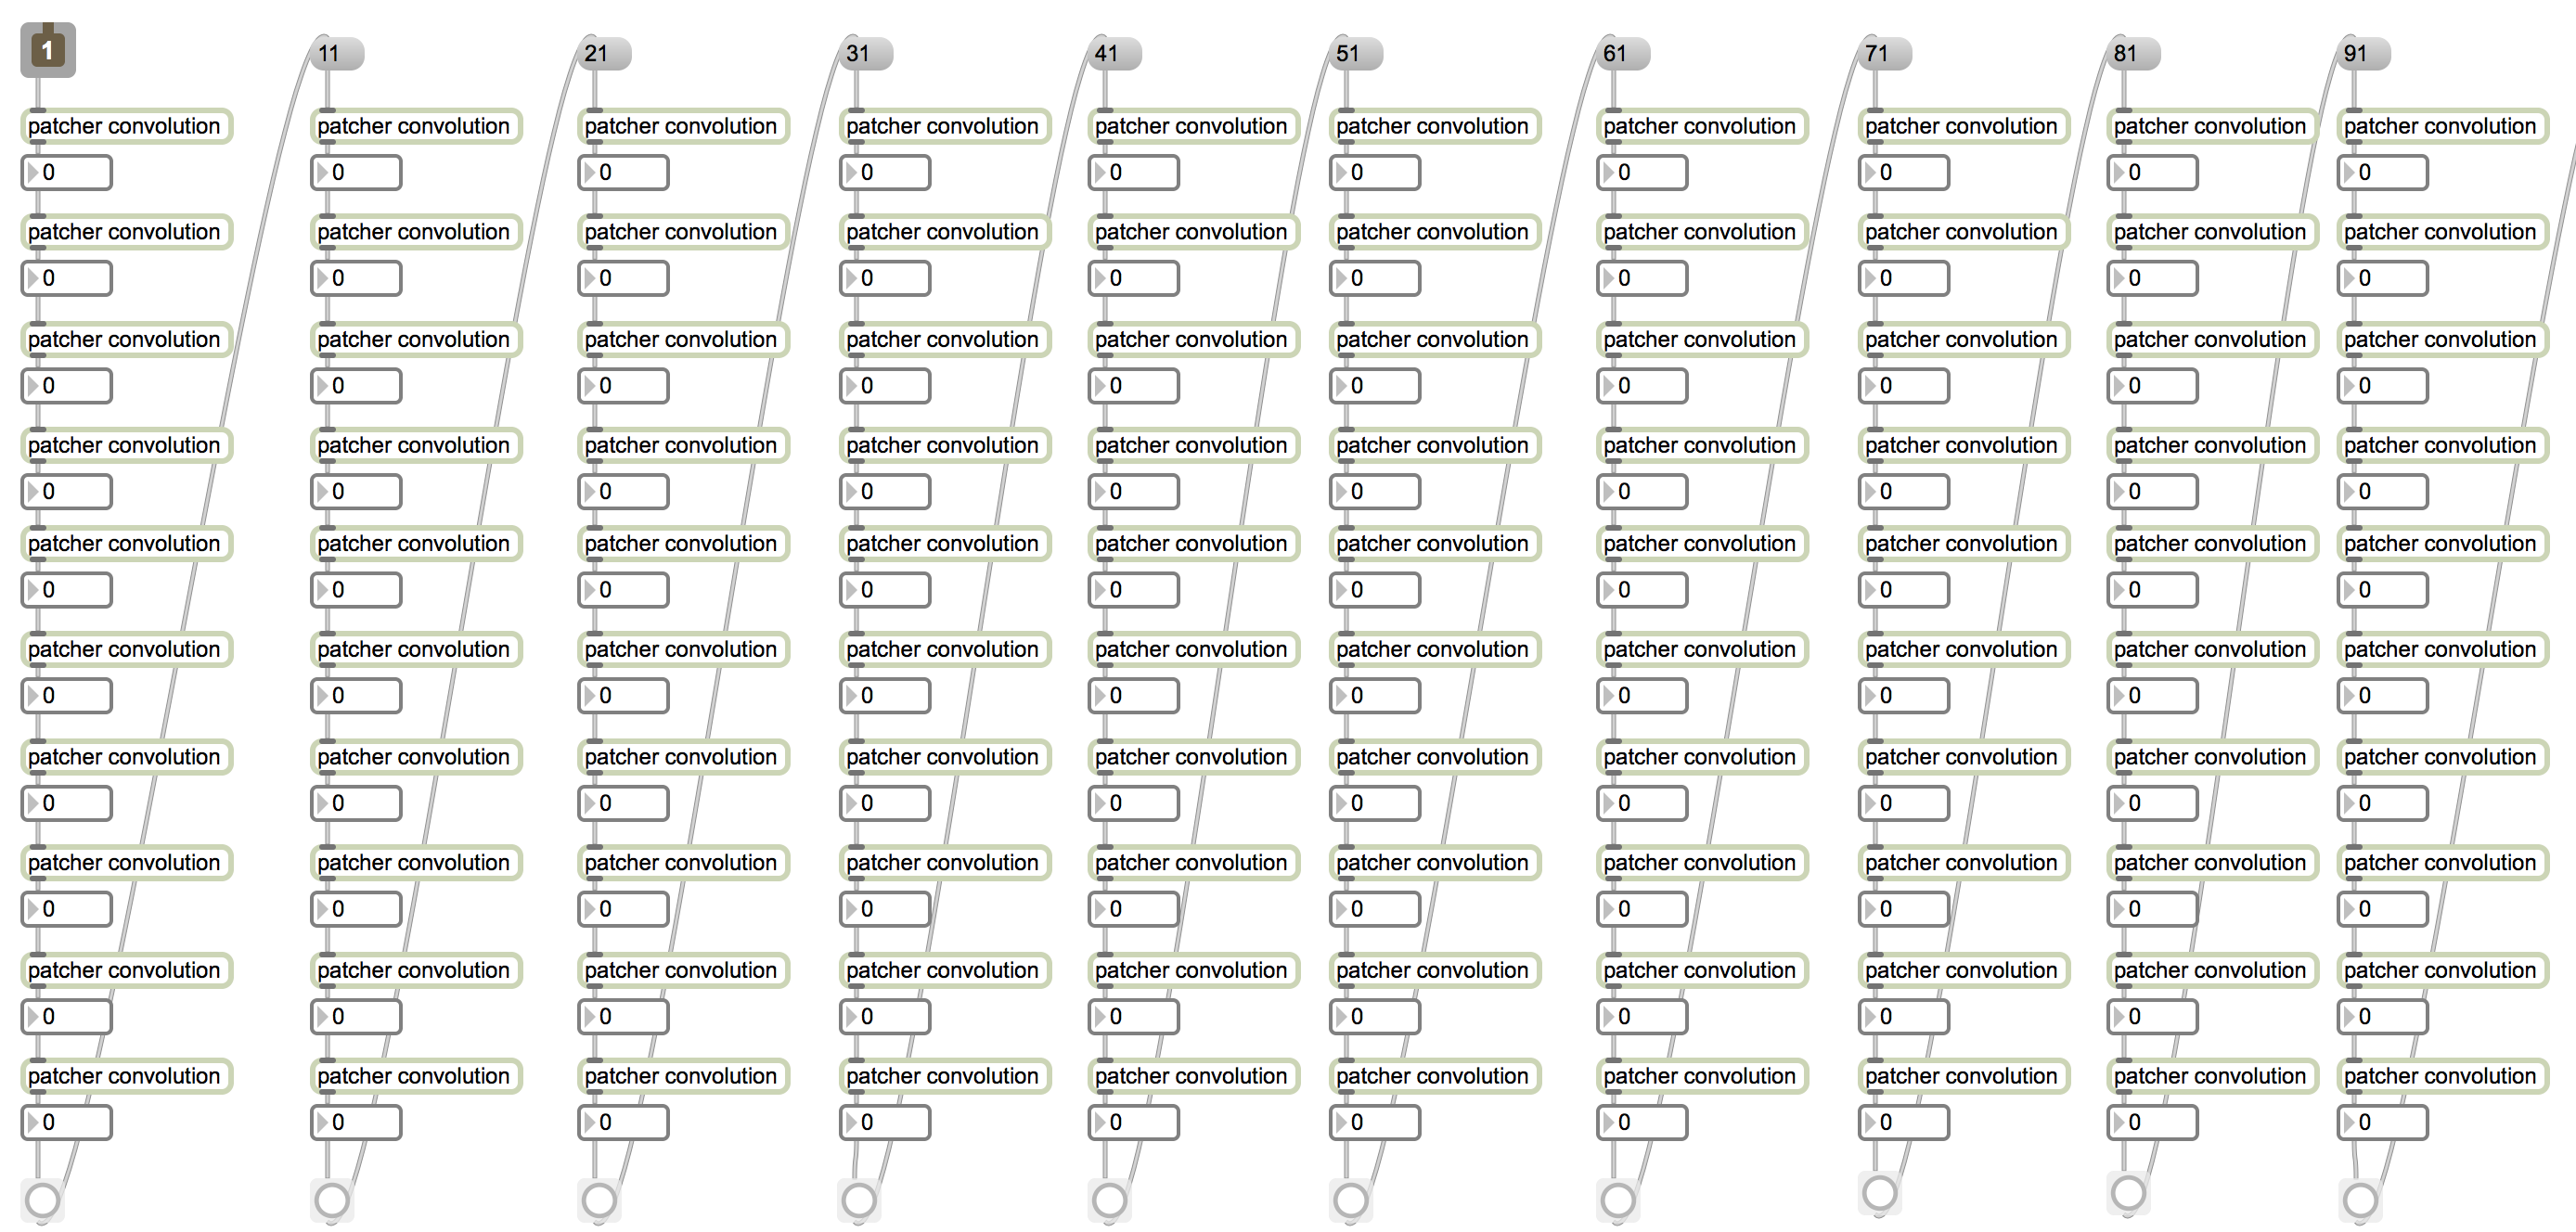
\includegraphics[scale = 0.4]{Sections/Implementation/Max/images/Max/Iteration2/preload.png}}
				\caption{Chained convolution patches used to pre-load each \ac{RIR} file. \textit{Image taken from Max 6 as the version of this patch would not run in Max 7}}
				\label{preload}
			\end{figure}


			Though it was possible to load smaller grids, such as a 9x9 grid used when locations are separated by 5m, the larger grids caused the system to run too slowly due to the amount of RAM that was used.

		 \paragraph{Iteration 3 (Final)}
		 \label{iteration3}
		 	%Path defining

		 	The previous iterations attempted to allow the user to move anywhere within the \ac{VAE} in real time as they moved their finger around the screen, however due to technological implications, this was not possible. It was therefore decided to find a compromise, where the user could draw themselves a path around the space and the system would move them along the path, one \ac{RIR} location at a time at a rate determined by a timer, allowing the system the load all appropriate files with ample time to prevent the system from lagging.

		 	The top half of figure~\ref{storeLocations} has been seen already in figure~\ref{locationsConvert}, however the bottom of figure~\ref{storeLocations} shows how the resulting file number is used. It gets sent to a javascript file that adds the file number to the end of a mutable array (an array that can be extended or truncated once created). As the file names are being stored, the corresponding files can be loaded when the system is ready, instead of trying to load them instantly as in~\nameref{iteration1}. Once the js object receivers a message from the timer (highlighted as number 3 in figure~\ref{myPatch}), the number at the start of the array is sent to the output. The array is then truncated by 1, moving the next file number to the front of the array waiting for the next timer message. If a reset message is sent to the third inlet of this js object (by pressing the first button in section 1 shown in figure~\ref{myPatch}), the arrays are cleared enabling the user to start drawing another path if the previous path had not been completely travelled.

		 	%-------------Store Locations Image-------------%
			\begin{figure}[H]
				\centerline{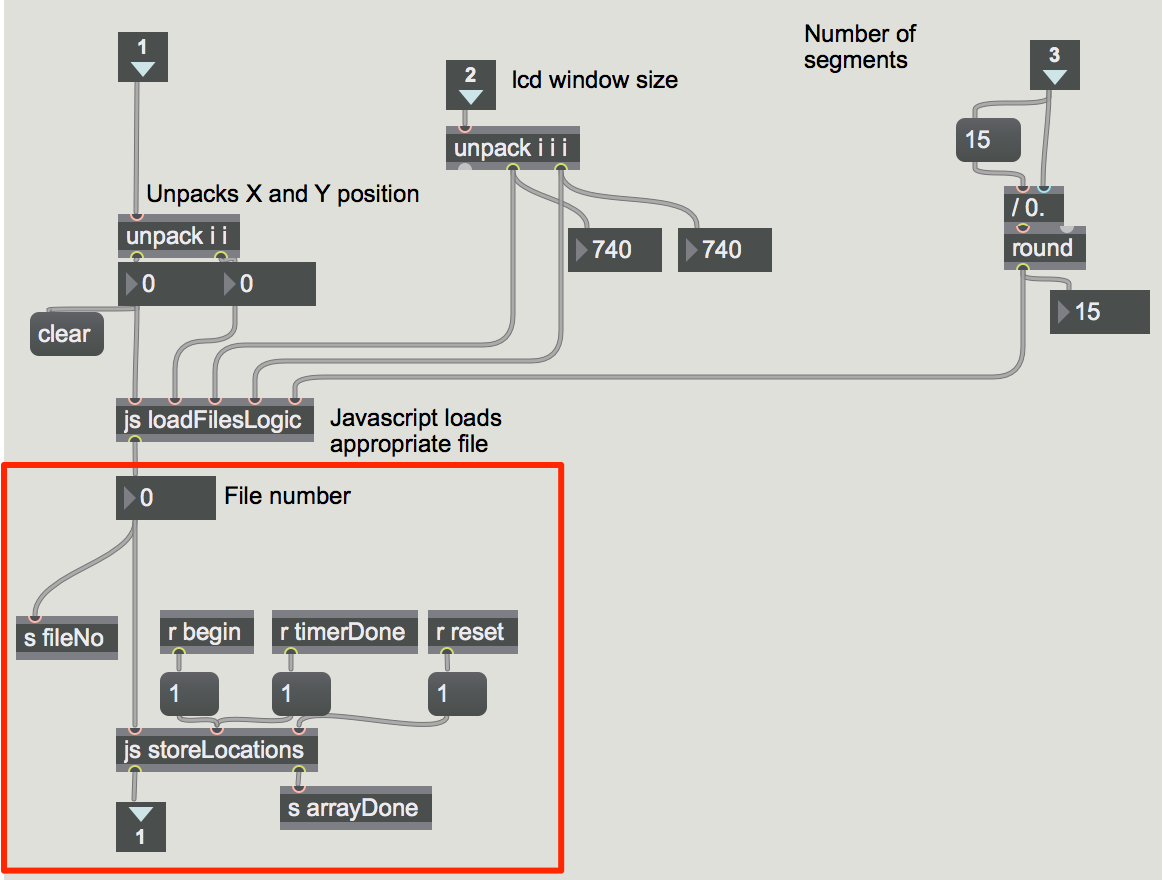
\includegraphics[scale = 0.6]{Sections/Implementation/Max/images/Max/Iteration3/storeLocations_edit.png}}
				\caption{Highlighting the section of `UI\_to\_file' that stores the file numbers and outputs them when a timer is done.}
				\label{storeLocations}
			\end{figure}

			Figure~\ref{overviewIteration3} shows the output from the `UI\_to\_file' patch in the red rectangle (the patch that contains the contents of figure~\ref{storeLocations}) running into a new javascript called `js switcher' in the blue rectangle. This simple script ensures that each new file number is sent to a different convolution patch (shown in the yellow rectangle). This means that while a new file is being loaded into one of the convolution patches, the other two can be used to pan between two pre-loaded positions. This is illustrated in figure~\ref{movementIllustration}\\

		 	%-------------Iteration3 Overview Image-------------%
			\begin{figure}[H]
				\centerline{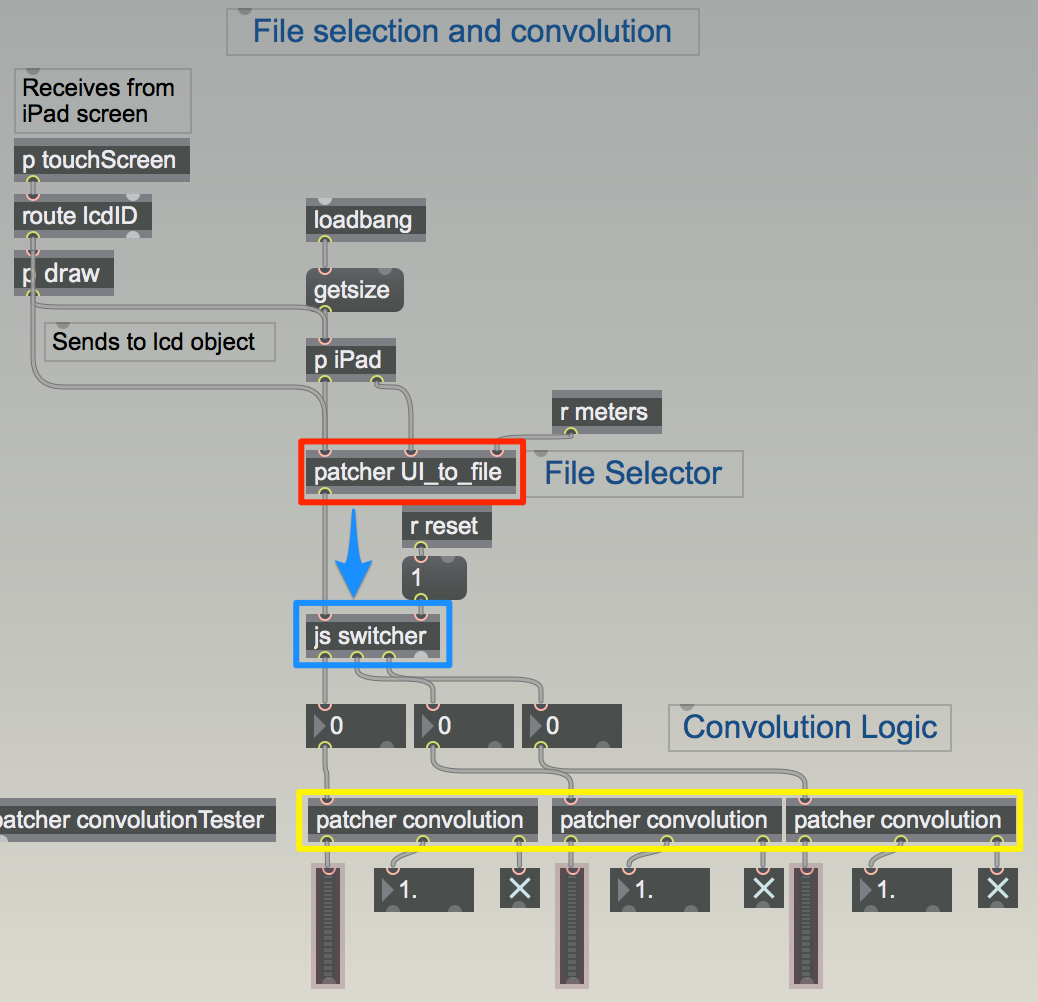
\includegraphics[scale = 0.5]{Sections/Implementation/Max/images/Max/Iteration3/fileSelectionConvolution_Edit.png}}
				\caption{\textbf{Red:} Outputs file stored file number. \textbf{Blue:} Distributed file number to a different convolution patch each time. \textbf{Yellow:} Receives file number and loades appropriate file into the system.}
				\label{overviewIteration3}
			\end{figure}


			%-------------Movement Illustration Image-------------%
			\begin{figure}[H]
				\centerline{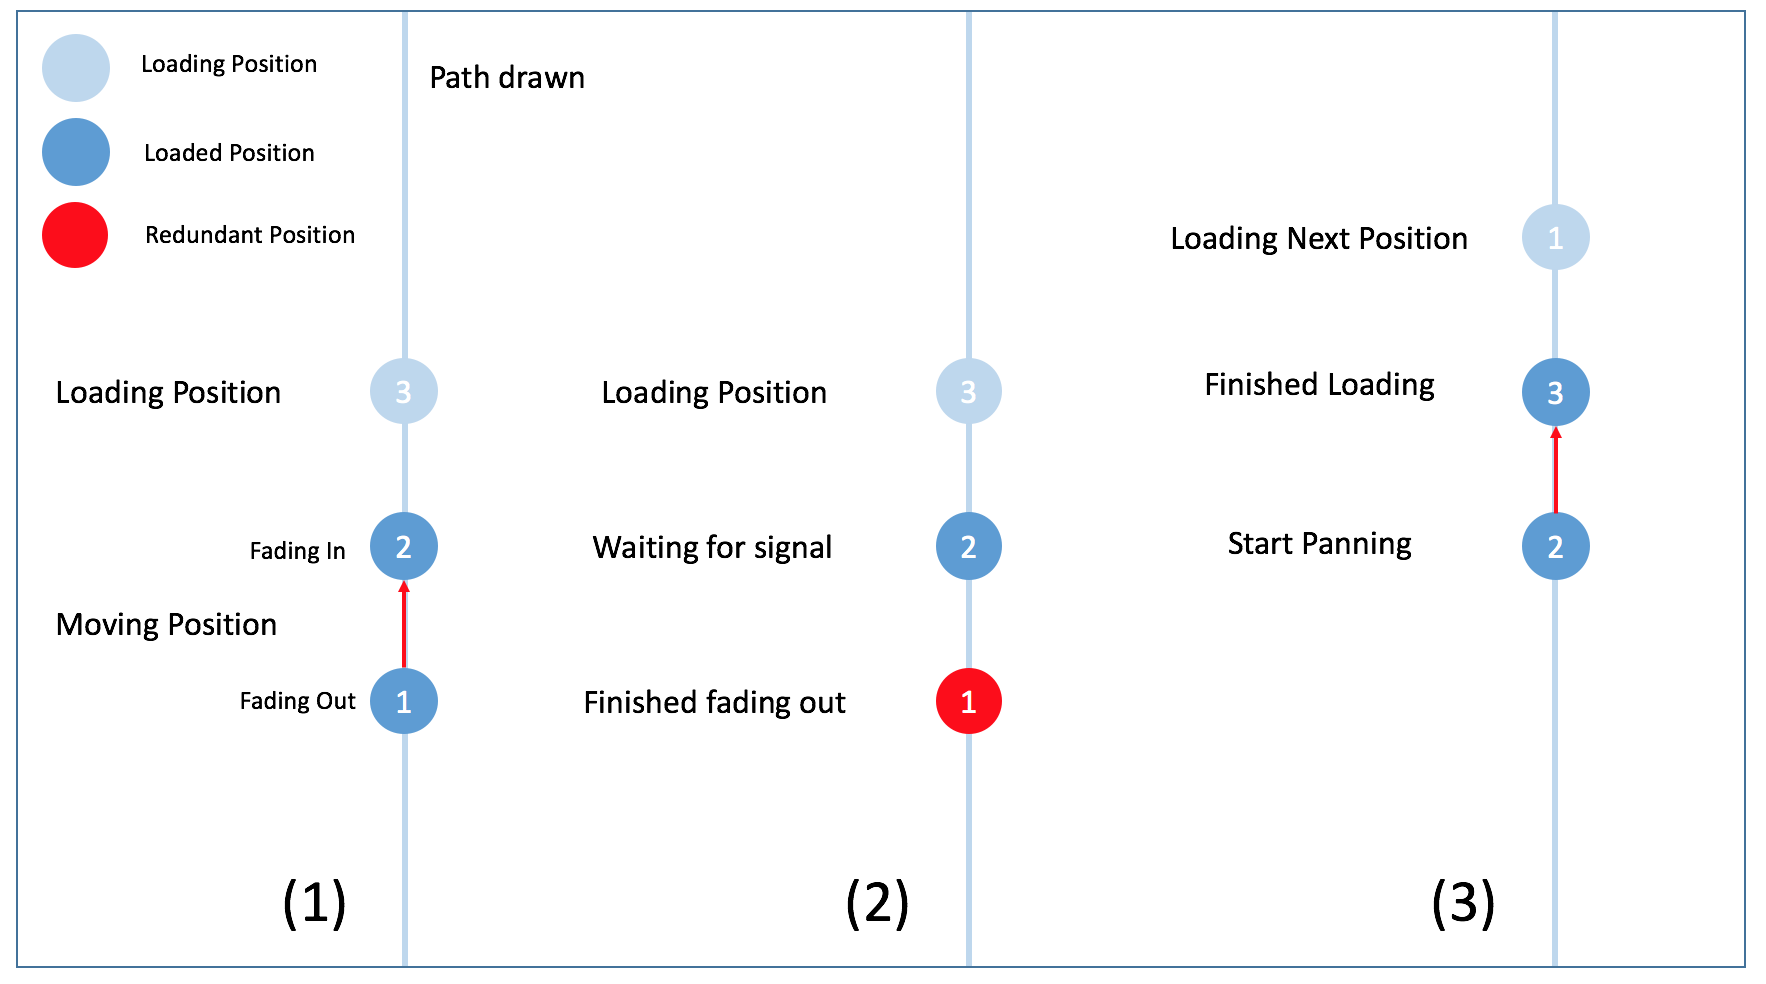
\includegraphics[scale = 0.45]{Sections/Implementation/Max/images/Max/Iteration3/movementIllustration2.png}}
				\caption{Illustration of how the three convolution patches work together to simulate movement, where the circles represent locations within the \ac{VAE} and are numbered to indicate which convolution patch they are loaded in. \textbf{(1)} User is moved between two loaded positions while the third patch loads a new \ac{RIR} fie. \textbf{(2)} The user is held in the new position until the next position has been loaded into the system. \textbf{(3)} User is moved between the two available positions while the next position is loaded into the system.}
				\label{movementIllustration}
			\end{figure}

			The convolution patches have three outputs connecting to:\\
			\textbf{1:} A level meter used to see which patch is being used.\\
			\textbf{2:} A number box to check the level of each patch. \\
			\textbf{3:} A toggle box used to see which spat convolution algorithms have been bypassed (a function that was later removed, explained in section \nameref{iteration3Issues}) These were used to monitor the functionality of the patch while testing.

				%-------------Convolution Patch Overview Image-------------%
			\begin{figure}[H]
				\centerline{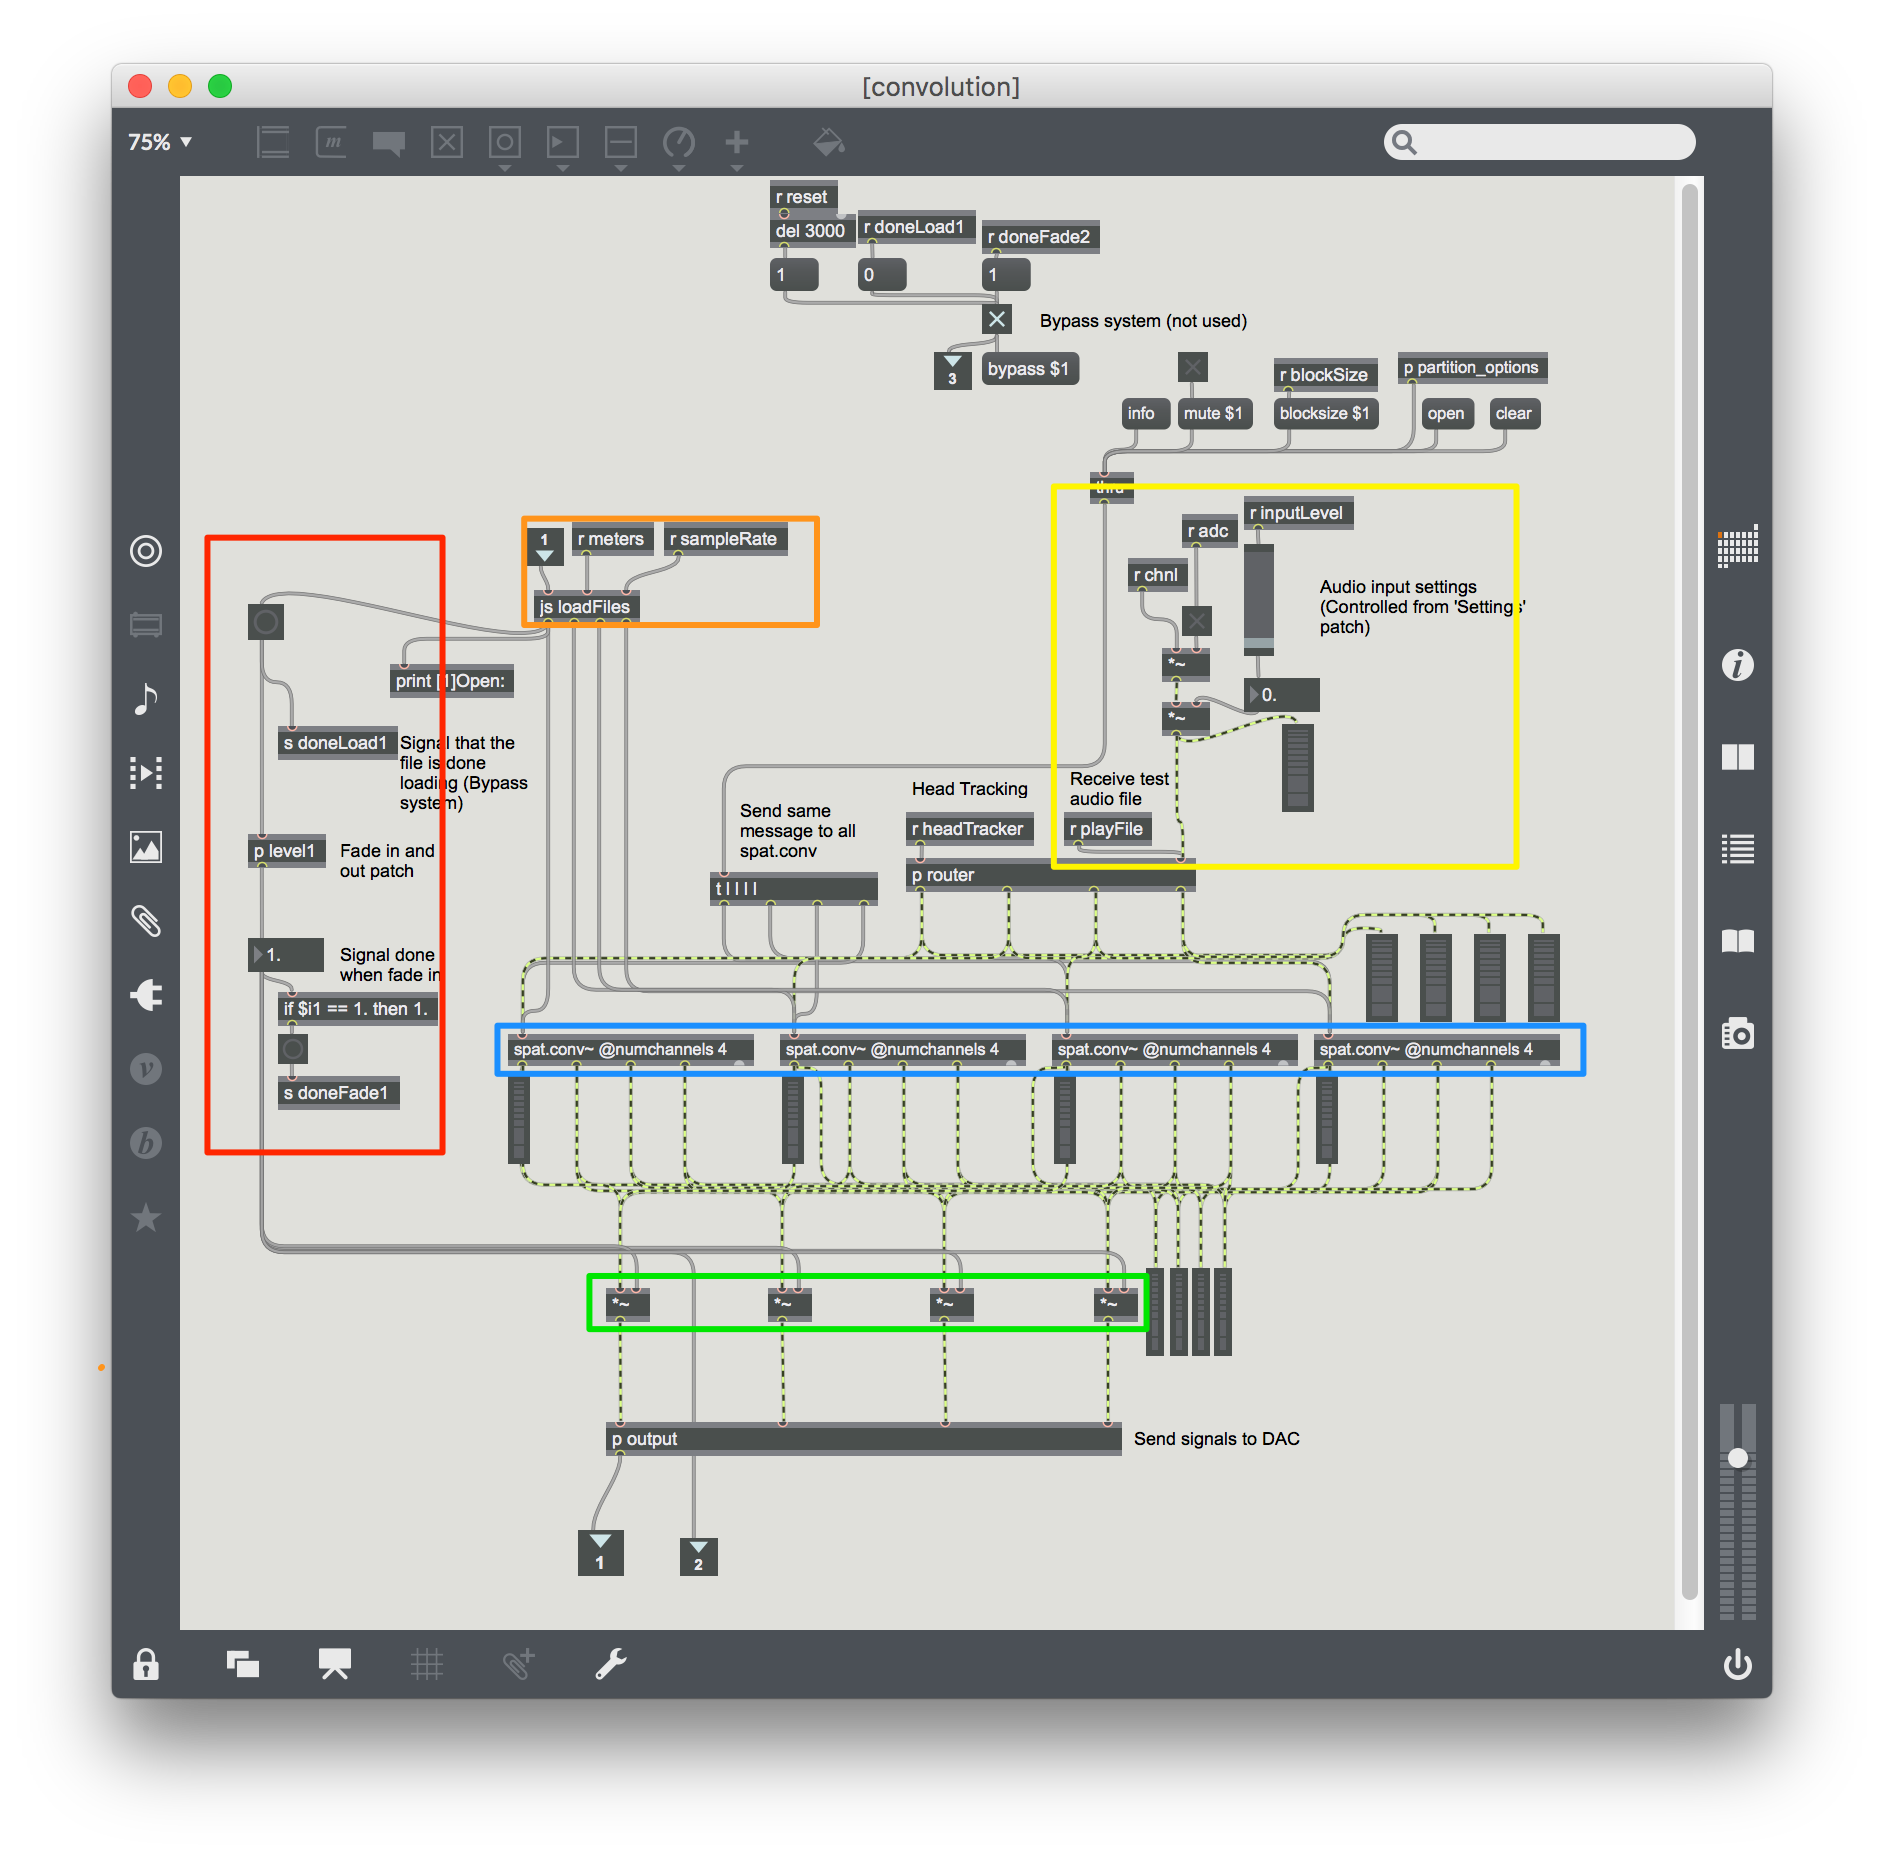
\includegraphics[scale = 0.5]{Sections/Implementation/Max/images/Max/Iteration3/convPatch_edit.png}}
				\caption{}
				\label{convPatch}
			\end{figure}

			To achieve the path following functionality, each convolution patch contains its own level control algorithm. Figure~\ref{convPatch} shows an overview of the first convolution patch which is a modified version of the original pathch used in the \ac{VSS}. The input to the convolution patch (orange) feeds the file number directly into a `loadFiles.js' javascript object. This simply prepends the number with the appropriate number of 0's (eg 1 becomes 001 and 28 becomes 028), then this number is concatenated with a file path pointing to where the audio files are located (see js file: loadFiles.js \textbf{LINK}). This outputs four `open' messages (one for each directional \ac{RIR} file)  followed by a file paths to the spat.conv objects (blue). These are the objects that actually search for the file and load it into the system. By sending the prepending `open' message, manually searching for a file is not required, thus automating the process. These objects convolve the loaded \ac{RIR} file with whatever audio input is given at its inlet, in this case the real time audio input or audio file (yellow). These outputs are then sent through multipliers (green), used to fade the signal in and out with an automated volume control (red).
		 	
		 	The automated volume controls receives a `bang' (signalling something has happened) when the `open' message is sent form the `loadFiles' js object (orange). This bang is also sent to the convolution patch that is currently at full volume. This prompts the volume of the current patch to increase while the volume of the previous patch decreases, thus panning between the two signal.


	\subsubsection{Location Tracking}
	\label{locationtracking}
	Figure~\ref{touchScreenPatch} shows the patch `touchScreen' which contains two main elements. The left side is used to draw a dot on the user interface that indicated to the user where they currently are in the virtual space and the right side is used to draw the user interface. Both are described in the following sections.

			%-------------Convolution Patch Overview Image-------------%
		\begin{figure}[H]
			\centerline{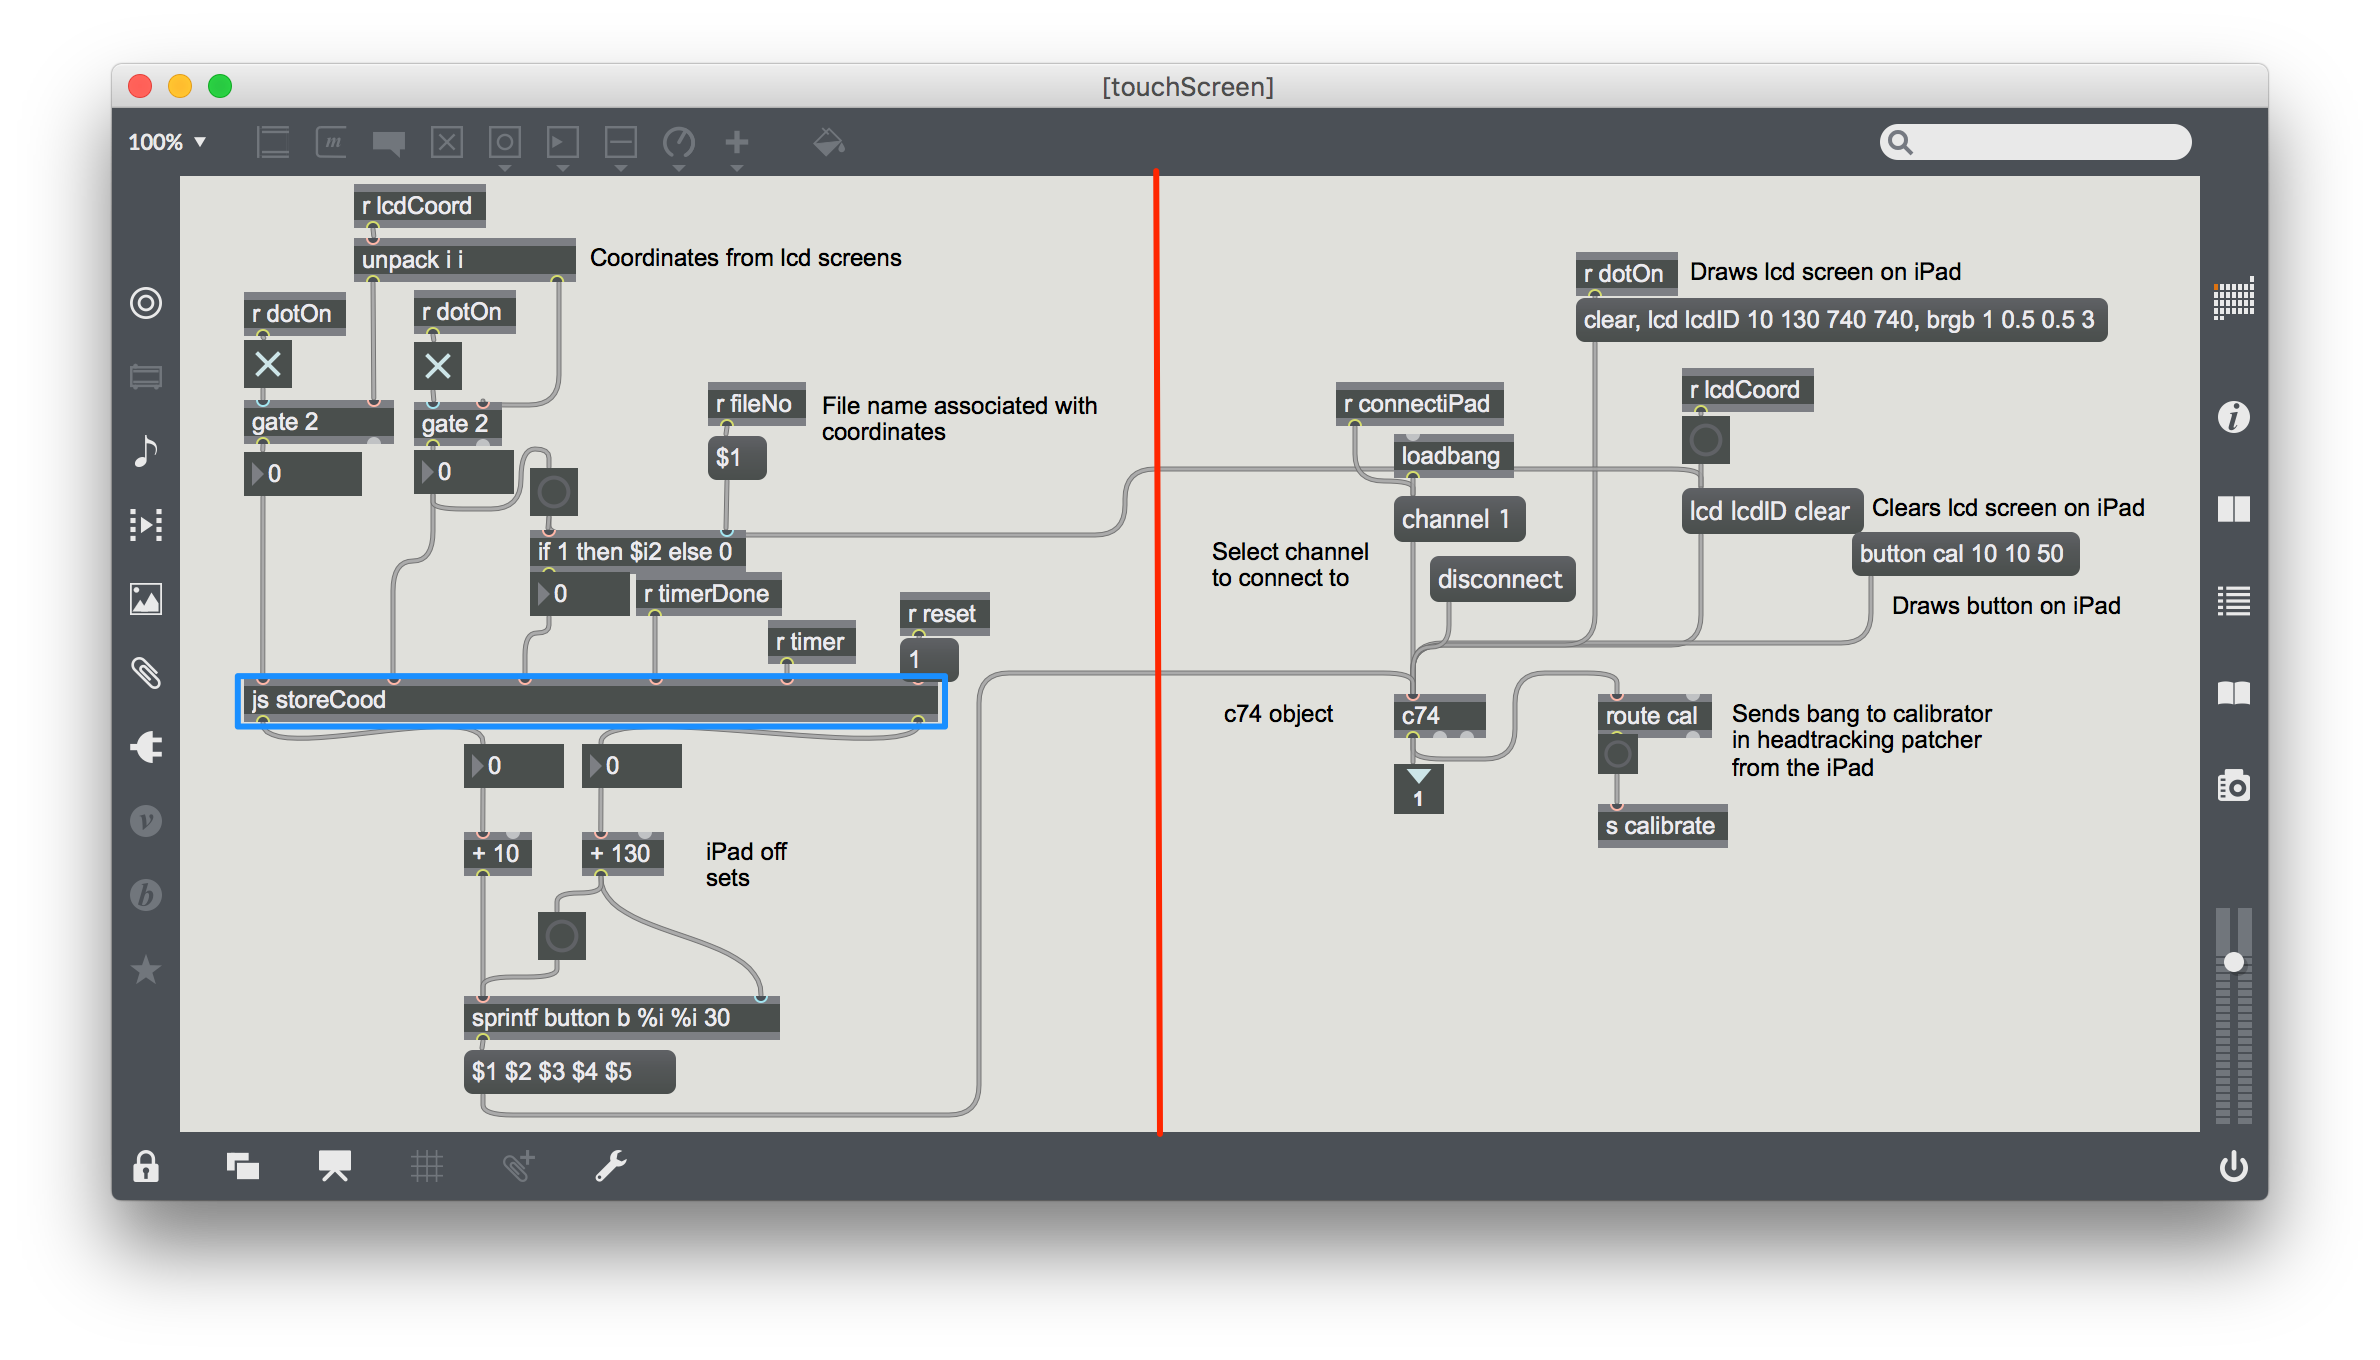
\includegraphics[scale = 0.5]{Sections/Implementation/Max/images/Max/UserInterface/pTouchScreen_edit.png}}
			\caption{Screen shot of `touchScreen', the patch used to produce the user interface on the iPad (right side) and to draw a dot on the iPad showing the user where they are located in the virtual space (left side). `storeCood' javascript object highlighted in blue.}
			\label{touchScreenPatch}
		\end{figure}

		\paragraph{User Interface}
			As previously mentioned, the c74 application was used to display a user interface on an iPad, allowing the user to select their location within the space. This is created on the right side of figure~\ref{touchScreenPatch}, by sending the `c74' object a message that contains the type of object that should be presented, its coordinates in the space as well as size and colour, the results of which are shown in figure~\ref{UIdot}. The output of the `c74' object returns information regarding the objects created in the user interface. In this case, the positions touched on the lcd screen will be sent from the iPad back to this `c74' object. This information is sent to the input of the `UI\_to\_file' patch. This allows the iPad screen to be used the same way as the lcd screen in Max is used (show previously in figure~\ref{lcd}).

						%-------------UI Image-------------%
			\begin{figure}[H]
				\centerline{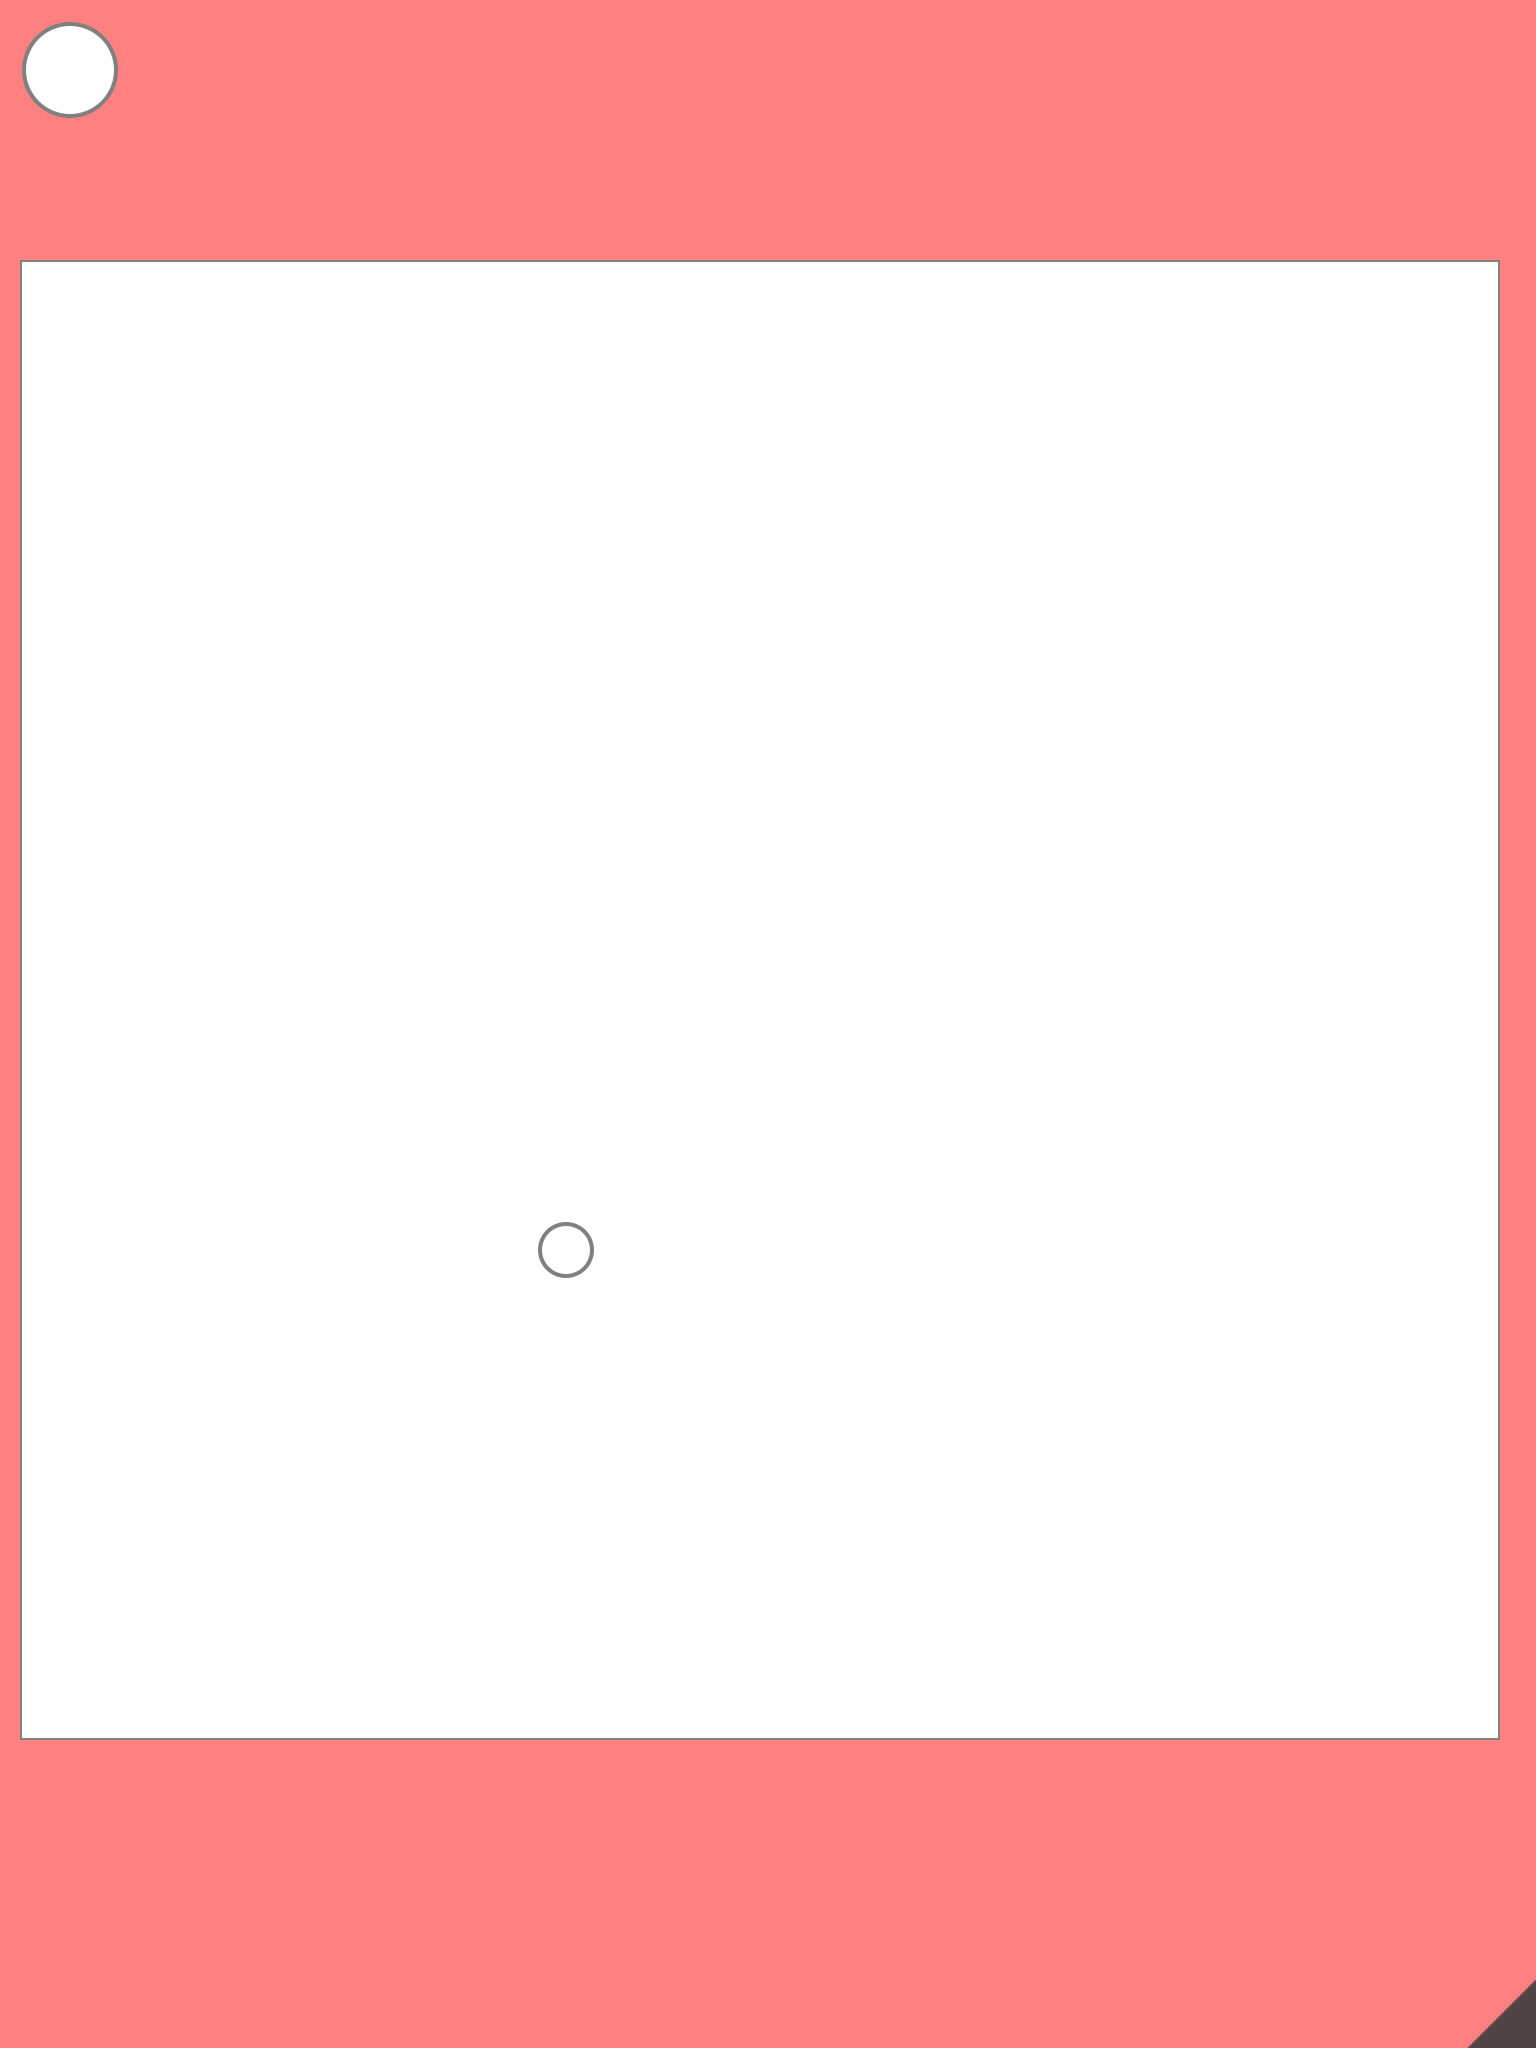
\includegraphics[scale = 0.15]{Sections/Implementation/Max/images/Max/UserInterface/UI_dot.png}}
				\caption{Screen shot of the user interface produced on the iPad. The large white rectangle represents the virtual space in which the user can place themselves, where the top of the rectangle is the front of the room (where the blackboards are in Hendrix Hall). The dot in the white rectangle is used to show the user where they are located in the space and the button in the top left corner is used for calibrating the head-tracking device.}
				\label{UIdot}
			\end{figure}

		\paragraph{Position Feedback}
			The left side of figure~\ref{touchScreenPatch} contains a javascript file called `storeCood' \textbf{Available here: LINK} (highlighted in blue) with a number of inputs. As mentioned above, the `c74' objects can retrieve data from the lcd screen on the iPad. When the user selects a location, the (x,y) coordinates are sent to the first two inputs of the javascript file respectively. These coordinates are stored in a list along with the corresponding section that they are located in (third input), calculated using the method described in section~\fullref{locationSelection}. Figure~\ref{locationsExample} shows a simple example, where the coordinates of a path spanning across 4 sections are stored in groups.

			Input 4 and 5 receive two different signals routed from the main timer (labelled 3 in figure~\ref{myPatch}). Input 4 receives a signal every time the timer is done (ever 2.5 seconds) and input 5 receives a message every 100ms (the rate at which the timer increments). These are used to call the two main functions that are used to output the coordinates at the correct times, \texttt{findLength()} and \texttt{outputCoords()}. Each time the timer finishes (after 2.5 seconds), \texttt{findLength()} starts from the beginning of the list of stored coordinates and scans through them, calculating how many coordinates are located in the same section. For the example in figure~\ref{locationsExample}, this would find a length of 2 for positions 1 and 2 located in section 5. As the user is moved to a new \ac{RIR} location every 2.5 seconds, \texttt{outputCoords()} will output the coordinates that were travelled in that section evenly within that amount of time. This is done by dividing 2500(ms) by the number of points within that section. For the example in figure~\ref{locationsExample}, this would be $2500/2 = 1250$. Therefore, every 100ms the function checks to see whether it is time to output the stored coordinates, meaning the coordinates of position 1 and 2 will be output at times 1250ms and 2500ms. If we were to continue with the example, the next three positions, 3, 4 and 5 would be output at times 833ms, 1666ms and 2500ms, thus evenly spreading out the movement of the dot on the user interface screen \textit{meaning the dot should travel around the path at a continuous rate instead of in staggered increments}. An example of the dot movement can be found \textbf{LINK TO DOT MOVEMENT VIDEO}.

			%-------------Locations example Image-------------%
			\begin{figure}[H]
				\centerline{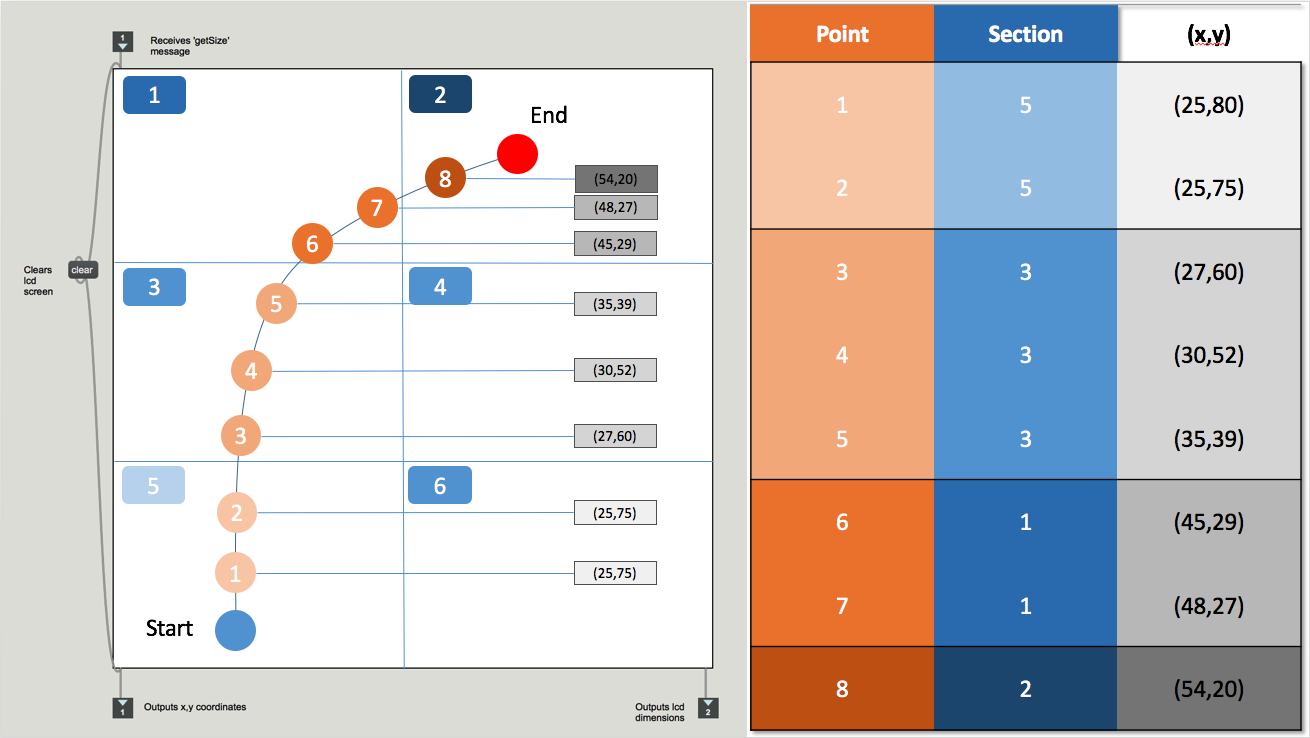
\includegraphics[scale = 0.4]{Sections/Implementation/Max/images/Max/UserInterface/locationsExample2.png}}
				\caption{Simple example of the coordinates along a path being stored in groups depending on which section of the lcd screen they are located. \textit{(The smallest number of sections possible is actually 9, but 6 are used here for simplicity)}}
				\label{locationsExample}
			\end{figure}

	\subsubsection{Head-Tracking}

		The original \ac{VSS} patch used an Oculus Rift as a head-tracking device which was also used to provide visuals of the \ac{VAE}. As this project does not provide visuals, a smaller, less obtrusive device was sought. Initially the YEI 3-Space Sensor \cite{YEI} was investigated, a small device that can track angular rotation and output results into Max. It was found however that the software used to interface between the device and the computer (a Mac) was only in a Beta stage. As a consequence, the output from the sensor did not function correctly or provide useful information.

		Instead, the c74 application already being used for the iPad user interface (see section~\fullref{locationSelection}) was used to extract rotational data from an iPhone. The iPhone data retrieved was accurate and provided a steady wireless connection, as opposed to the USB connection required for the YEI sensor. For user testing, a low-tech head-mounting solution was found by wrapping the iPhone in the front of a cotton hat. This was integrated with the existing head-tracking by creating a new patch that reads data from the iPhone (much like the patch used for the iPad) and maps the data to an angle from 0\textdegree~to 360\textdegree, including a calibration system ensuring that each user is facing the same way in the \ac{VAE}. The output of this was sent to the input of the existing head-tracking system where the Oculus rift data would have been sent. This data is used to pan between the four direction \ac{RIR} files simulating the effect of turning the the \ac{VAE}.

	\subsubsection{Settings Menu}

	Figure~\ref{settings} shows the settings patch `settings'. This can be used to determine which \ac{RIR} grid to use by selecting the number 1-5 on the top left of the patch (green buttons) as well as the sample rate of the \ac{RIR} files. The audio input settings can be used to change which audio input is used. The panning settings determine the speed at which the user is moved between \ac{RIR} locations.

		%-------------Locations example Image-------------%
		\begin{figure}[H]
			\centerline{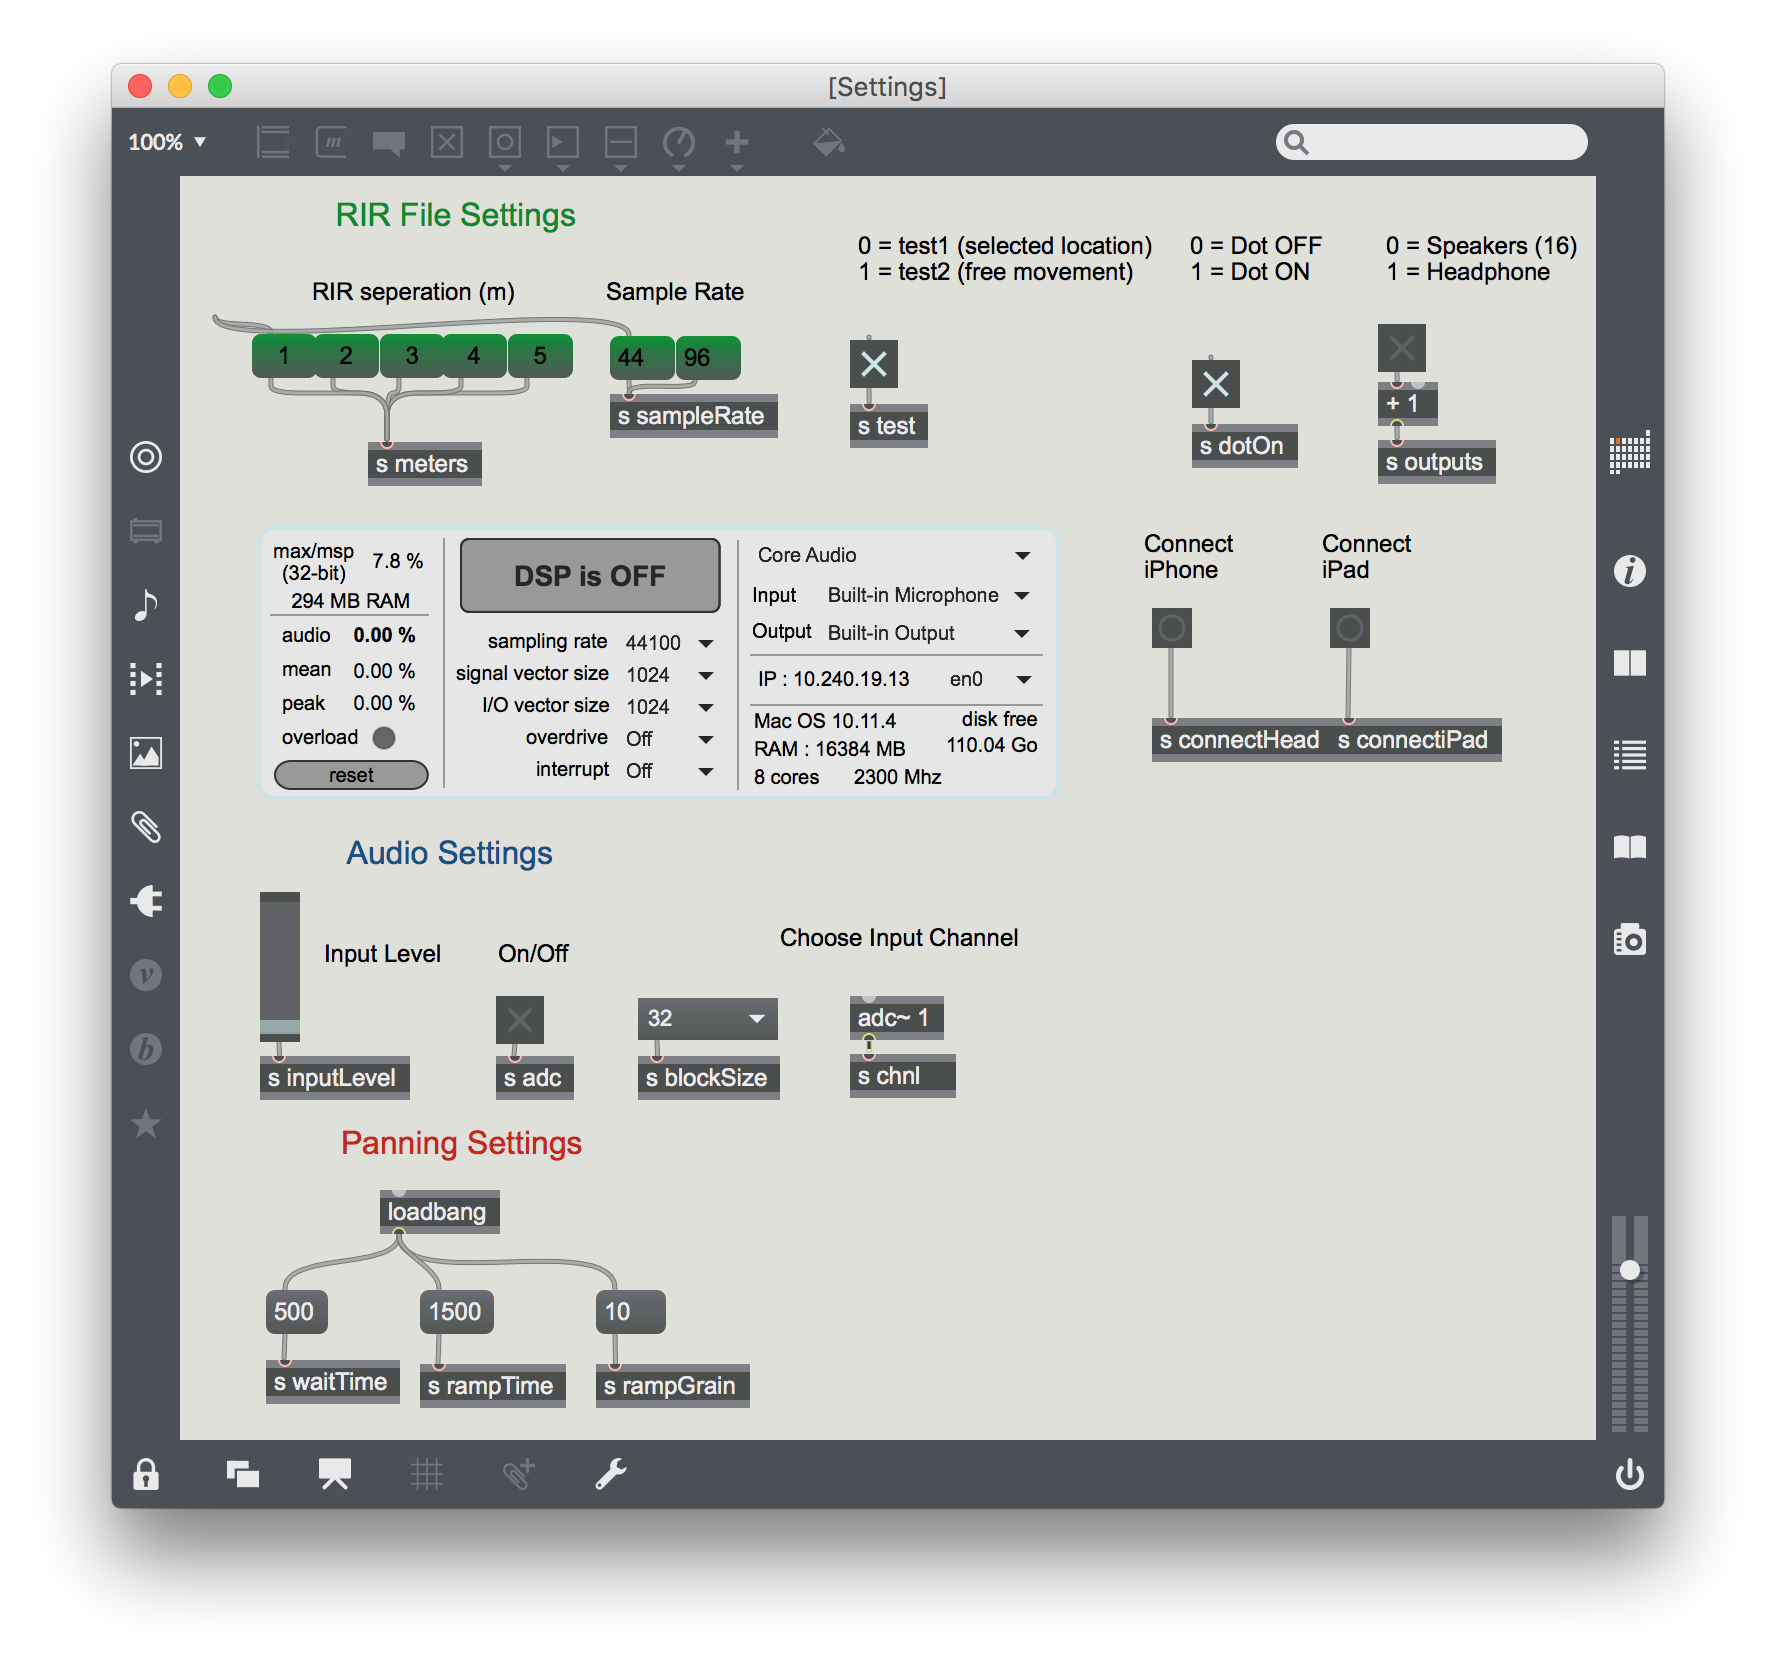
\includegraphics[scale = 0.4]{Sections/Implementation/Max/images/settings.png}}
			\caption{Settings patch used to control parts of the overall patch from one location}
			\label{settings}
		\end{figure}

		\subsubsection{Software Issues}
	\label{iteration3Issues}

		%Zigzag movement
		One issue raised when implementing iteration 3 was the way in which the user is moved through the virtual space. As only two \ac{RIR} locations are used at a time as opposed to using 4 \ac{RIR} locations for interpolation, the user is moved in a `zigzag' pattern. Figure~\ref{iterationMovement} shows two images illustrating how the user is moved through the virtual space using the final iteration of the software against the initial two iterations, where the curved blue line represents the path drawn by the user. The image on the right shows how the 4 \ac{RIR} locations are used together to make it sound like the user is placed between them. The image on the right shows how the user is passed between locations one at a time, causing the `zigzag' pattern.


		%-------------Latency Diagram-------------%
		\begin{figure}[H]
			\centerline{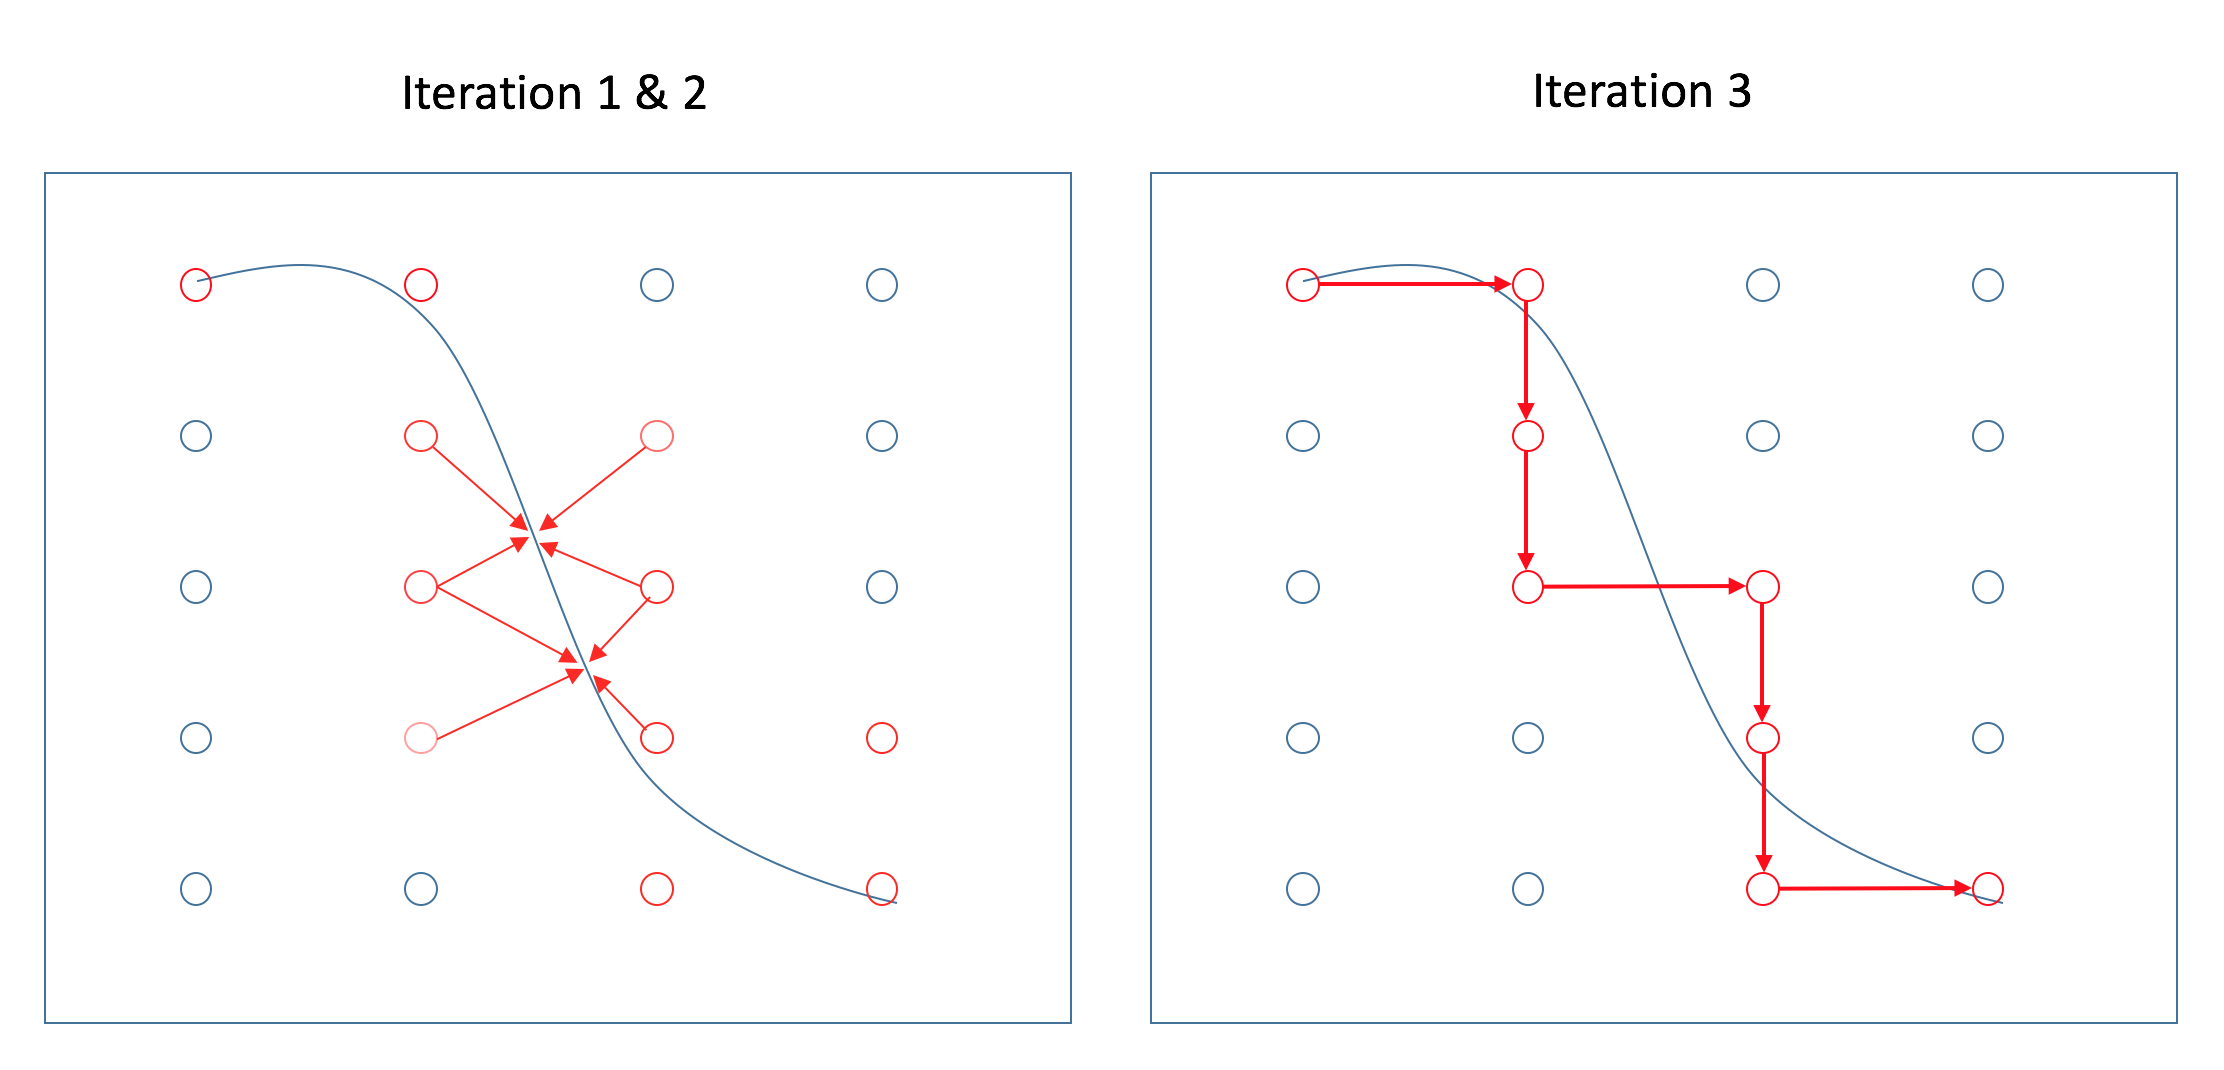
\includegraphics[scale = 0.4]{Sections/Implementation/Max/images/Max/iterationMovement.png}}
			\caption{Illustration of how the user is moved through the virtual space using different numbers of \ac{RIR} locations where the image on the \textbf{left} shows how 4 \ac{RIR}'s are used at a time and the image on the \textbf{right}  shows the user being passed between two \ac{RIR} locations at a time. The blue line represents the paths drawn by the user and the circles represent \ac{RIR} locations.}
			\label{iterationMovement}
		\end{figure}



		As previously explained in section~\fullref{iteration3}, three convolution patches were used to move the user between two \ac{RIR} locations while the third loads the next location. In an attempt to make the system less computationally expensive, if any of the convolution patched were loading a file as opposed to convolving an audio signal with one, the convolution algorithm was bypassed. However it was found that any delay in turning the bypass on or off produced a `popping' noise. Small delays in turning the bypass on and off often occurred, therefore this bypass functionality was removed.


	\subsection{Latency}

		The time taken for the input signal to run through the system causes the room reflection to arrive at the user at the incorrect times. To determine the length of the delay, a latency test was conducted. The test procedure was similar to that in the production of the original \ac{VSS} \cite{Brereton2014} with some slight differences. Two Earthwork M30 reference microphones \cite{earthworks} were placed in the centre of the speaker array. One was connected to the input of the max patch and the other was connected to a Mac running reaper through a MOTU audio interface \cite{motu} to record a reference input. An output channel running to one of the Genelec speakers was routed to the second input of the MOTU interface. This was used to record the signal after it had run through the Max patch, thus allowing the two signals to be compared to find the latency time. Both systems were running at a sample rate of 44.1kHz. To identify the impulse clearly, a pair of drumsticks were used to produce an impulse. This was then convolved with a 4-channel Dirac impulse (1 sample of amplitude 1) of approximately 3 seconds long. Figure~\ref{latencyDiagram} shows a diagram of the latency measurement process.

		%-------------Latency Diagram-------------%
		\begin{figure}[H]
			\centerline{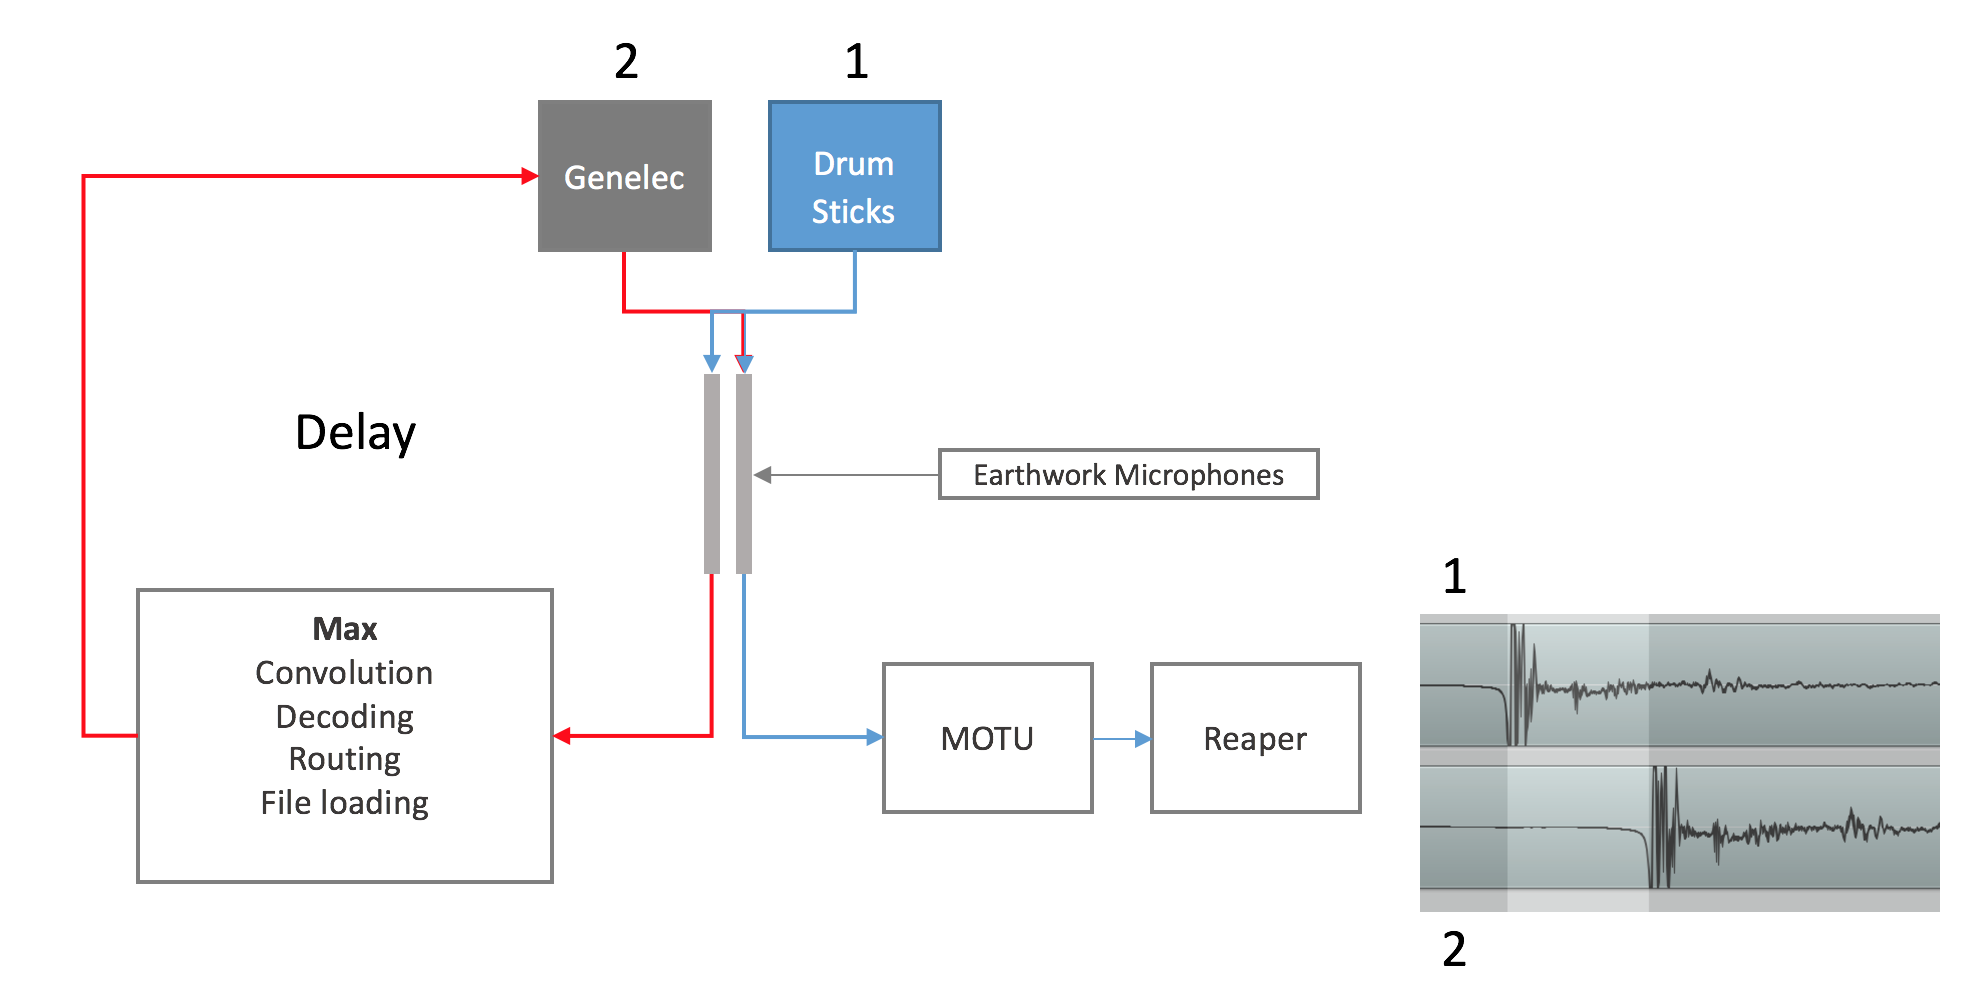
\includegraphics[scale = 0.4]{Sections/Implementation/Max/images/Latency/latencyDiagram.png}}
			\caption{Diagram showing the latency measurement process. Red arrow shows the signal being delayed due to running through the max patch, eventually being output from the Genelec and running into reaper. Blue arrow indicates the direct signal to Reaper. The numbers indicate which of the audio waves comes from which source, 1 being the direct sound and 2 being the delayed sound.}
			\label{latencyDiagram}
		\end{figure}

		Previous testing of the system had shown that the system ran smoothly when using an input block size of 32 in Max, however for future records (and in case the system speed were to slow down due to potential future changes) the latency was measured for varying block sizes. The following table shows the resulting latency time due to the different block sizes used in Max. The total latency is calculated by adding 5ms to the system latency. This accounts for the time taken to travel from the loudspeaker to the centre of the speaker array where the user will be present.


		\begin{center}
		\begin{tabular}{|c |c |c |c|}
		\hline
		Sample Rate (kHz) & Block Size & System Latency (ms) & Total Latency (ms) \\ \hline
		44.1 & 512 & 27 & 32 \\ \hline
		44.1 & 256 & 20 & 25 \\ \hline
		44.1 & 128 & 18 & 23 \\ \hline
		44.1 & 64 & 17 & 22 \\ \hline
		44.1 & 32 & 17 & 22 \\ \hline
		\end{tabular}
		\end{center}


	\subsection{RIR Trimming}
	\label{RIRtrimming}
		Due to the latency present in the system, the first 22ms of the \ac{RIR}'s had to be trimmed. Figure~\ref{odeonTrim} shows two of the synthetic \ac{RIR}'s, the top shows one from the centre of the room (8.85m from the left wall) and the bottom shows an \ac{RIR} taken 1.85m away from the left wall which are two of the locations that were also taken in Hendrix Hall for user test \#1. Both of the \ac{RIR}'s being analysed were produced with the sound source facing the left wall to emphasis the early wall reflection making the following point more obvious. 

		Points (1), (2) and (3) are identical in both \ac{RIR}'s showing the start of the impulse, the direct sound and the floor reflection respectfully. The main difference in the \ac{RIR}'s are the direct reflection times from the left wall. (4) shows the wall reflection occurring at 0.04084s, indicating a travel distance of 3.75m (following the same patch described in figure~\ref{reflectionPaths} in section \fullref{odeon:results}). (5) shows the reflection from the same wall, however occurring much later due to the greater distance from the wall. The point at which the \ac{RIR}'s will be trimmed is indicated by the red intersecting line, occurring at approximately 0.052s. It can be seen that the direct reflection from the left wall (4) is removed from the impulse, whereas in the \ac{RIR} in the centre of the room, the direct wall reflection (5) remains in the trimmed version of the \ac{RIR}. Due to the 22ms delay, any sound that travels less than 7.568m (if the source and receiver were placed 3.784 away from a surface) before reaching the receiver will be removed from the \ac{RIR}. 

		The necessity for direct sound has been previously discussed in \cite{Devore2009}, stating that as reverb builds up over time eventually masking reflections, the direct sounds are used for sound source localisation. As the user in the \ac{VAE} is both the sound source and the receiver, they will rely on direct reflections from the walls to determine their location within the space, however, the direct reflections from walls have had to be removed in some cases. Therefore, when moving closer to a wall, it may become difficult for the user to determine their locations.

		%-------------Latency Diagram-------------%
		\begin{figure}[H]
			\centerline{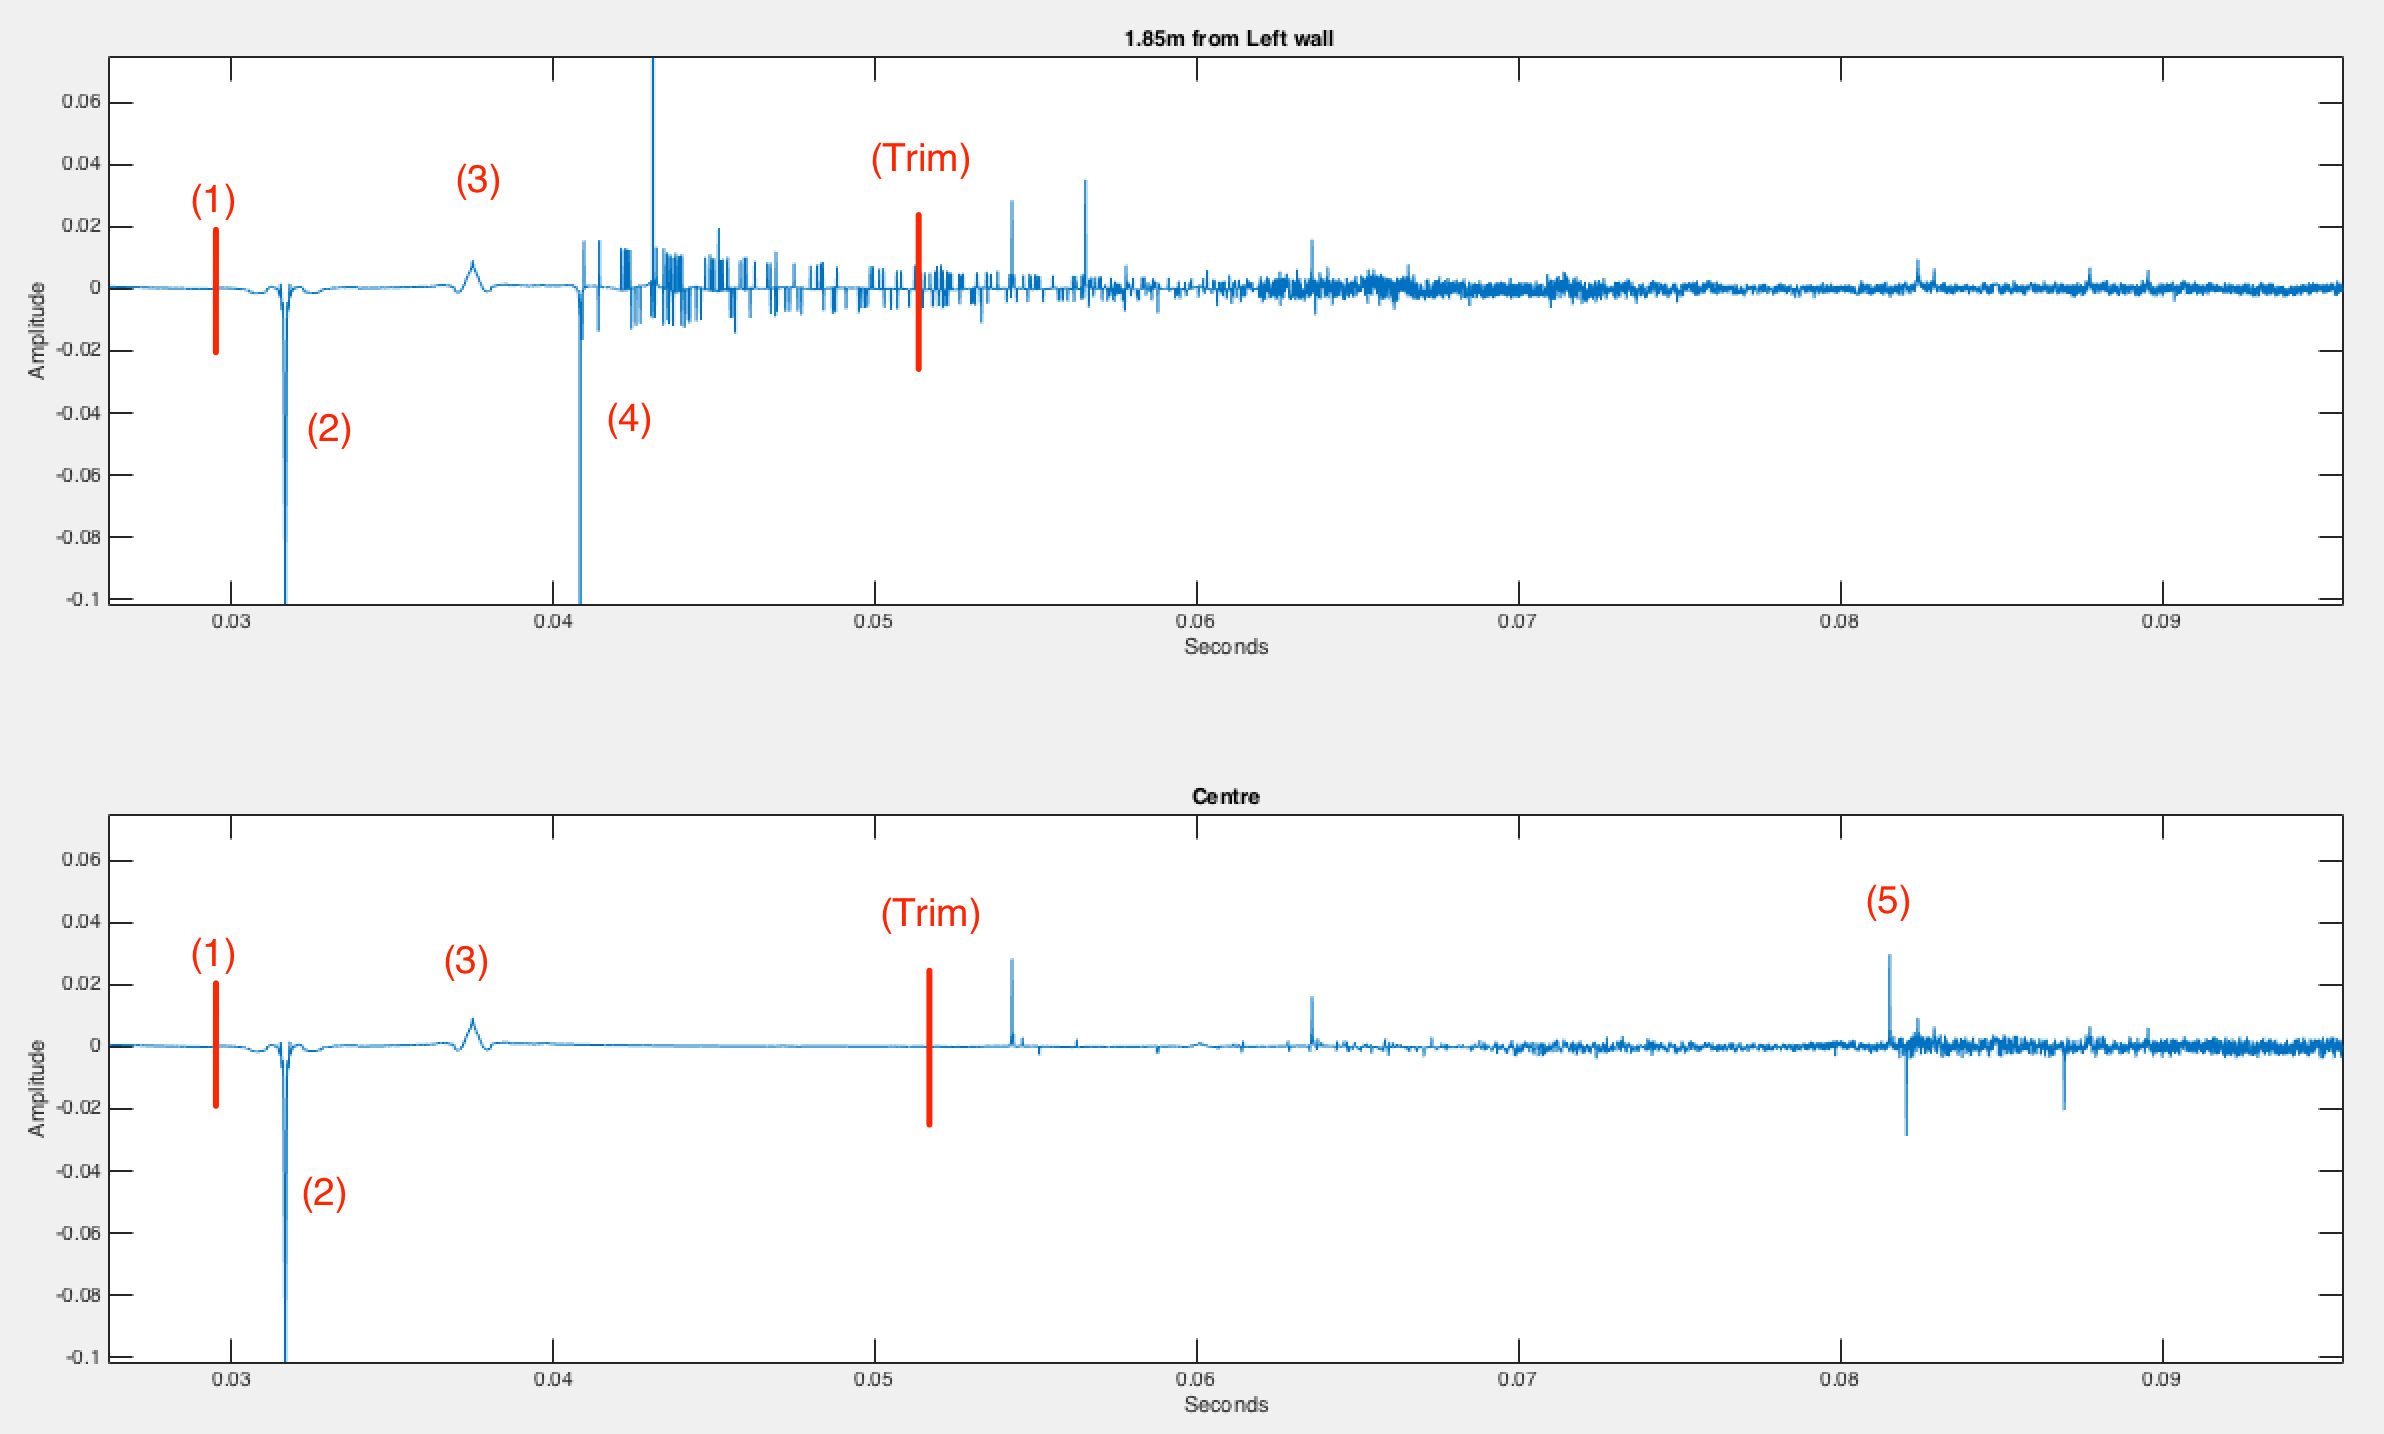
\includegraphics[scale = 0.4]{Sections/Implementation/Max/images/Latency/odeonLatency_edit.png}}
			\caption{}
			\label{odeonTrim}
		\end{figure}

		The Matlab script used from audio file trimming can be found: RIRtrim.m


		
		% This was done for the real \ac{RIR} measurements as well. Figure~\ref{realTrim} shows two \ac{RIR}'s in the same positions as mentioned above, where the early wall reflection in the bottom \ac{RIR} (3) is trimmed.

		% 	%-------------Latency Diagram-------------%
		% \begin{figure}[H]
		% 	\centerline{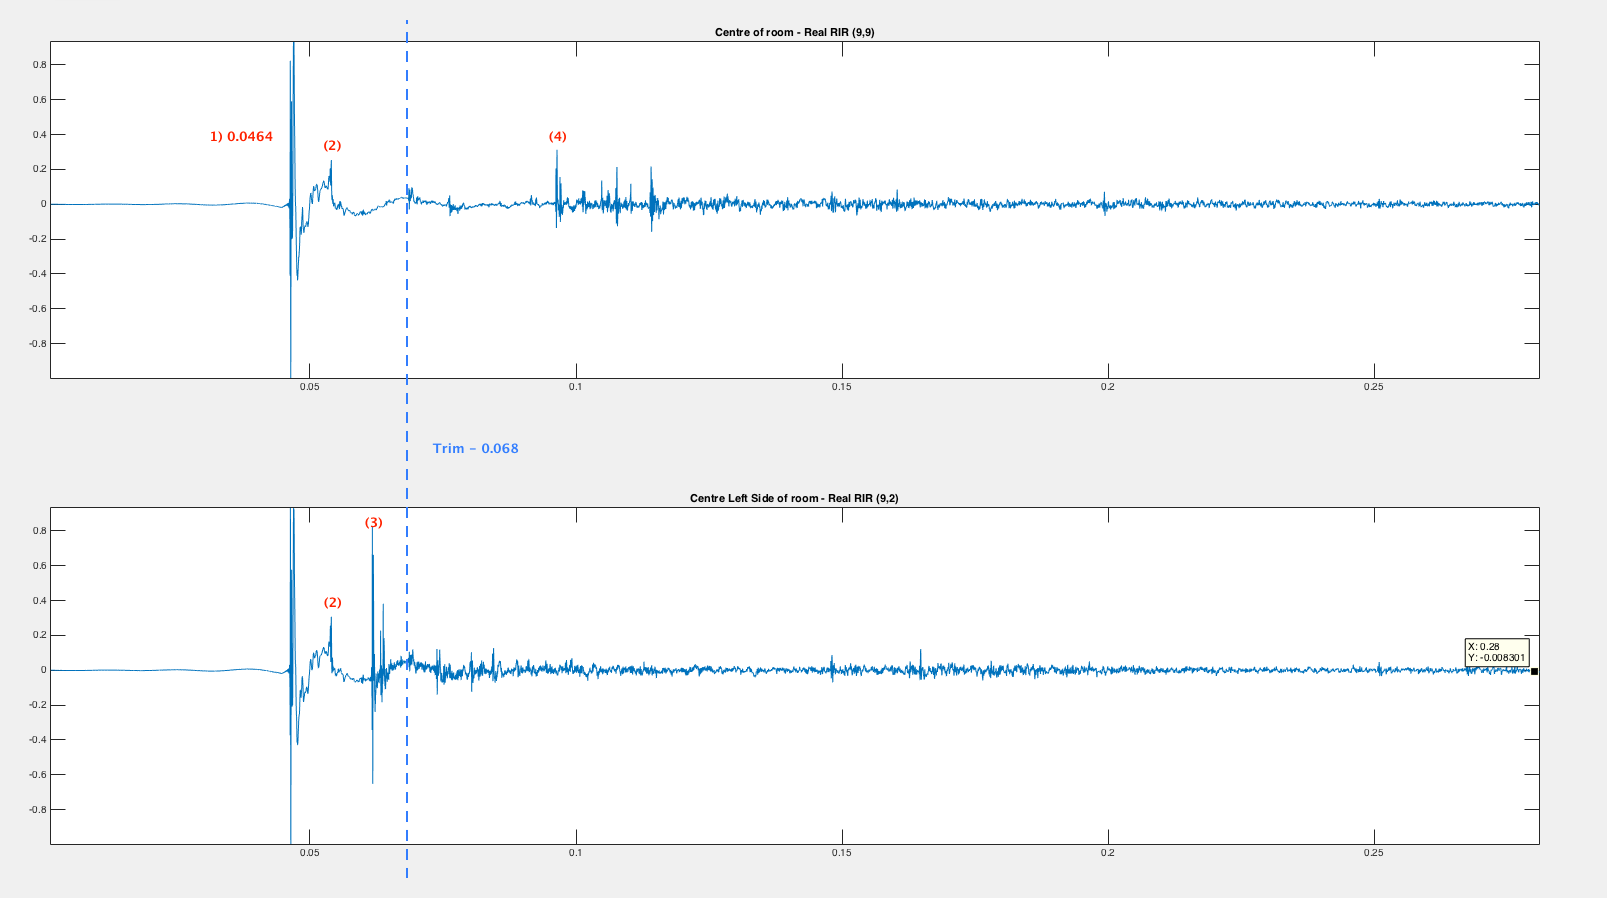
\includegraphics[scale = 0.2]{Sections/Implementation/Max/images/Latency/RealRIR(9,9)(9,2)_90.png}}
		% 	\caption{}
		% 	\label{realTrim}
		% \end{figure}

	\subsection{Software Implementation Summary}

		Revisiting the aims regarding software implementation set in \fullref{background:aims}, it can be said that two out of the three accomplished:

		\textbf{1)} The production of a user interface that can be used remotely from within the spherical speaker array. 

		\textbf{2)} The extension of the Max patch that could accommodate the user interface and load the appropriate \ac{RIR} files required to place the user in the desired location within the \ac{VAE}. 

		These has been achieved by producing the user interface using the `c74' object, allowing the iPad to communicate with the Max patch and visa versa. The interaction with the user interface is interpreted by the `UI\_to\_file' patch and the `loadFilesLogic' javascript object. These successfully interpret the users intention to move to a position within the \ac{VAE} and calculate the appropriate files to load.
 
 		\textbf{3)} The production of a system that can interpolate between the appropriate \ac{RIR} positions.

 		For the third aim set, it must be said that this was only partially fulfilled. Though the final iteration of the software (\fullref{iteration3}) interpolates between the appropriate \ac{RIR}'s for the given design, it does not work the way originally intended due to the technological restrictions previously stated. Instead of allowing the user to `freely' move around the space, they are instead restricted the the available \ac{RIR} locations and are only able to move between them when moving from one set location to another, as opposed to being able to hover between them as would have been able using iteration 1 (\fullref{iteration1}).

 		However, as the user interface interpretation section of the software simple outputs the required file names, it can be integrated with an improved version of the mobility section in the future. Therefore with simplifications to the first iteration of the software, such as providing the user with a grid of four \ac{RIR} locations instead of a full grid of 9, though less accurate, would be much quicker and would provide more freedom than the currently implemented version.

		%The latency due to the system running in real time degrades the ability to access localisation
		Due to this being a real time system, the latency introduced as a result greatly effects a large number of the \ac{RIR} files being used by having to cut 22ms of each one of them. This unfortunately removes some of the direct wall reflections for surfaces that are closer than 3.75m. However, this process also removed the direct sound and floor reflection as desired.




		

\end{document}